\section{Errors, Orchestration and Synchronization}
\label{chap:correctness_evaluation:categorization}

\mnote{Context: categorization and synchronization}
In \autoref{chap:errors}, we have presented and discussed a categorization of errors in transformation networks.
Such errors can occur when different kinds of mistakes are made when developing transformation networks, especially missing synchronization of the individual transformations, as discussed in \autoref{chap:synchronization}, but also because an algorithm that applies the transformations is not able to find consistent models because of the orchestration problem, as discussed in \autoref{chap:orchestration}.

\mnote{Empirical evaluation of categorization and synchronization}
We empirically evaluate different aspects of errors, their categorization, and their avoidability as well as resolvability by the proposed approaches in a case study.
In that case study, we utilize a set of independently developed transformations, which were not supposed to be used in a transformation network.
In consequence, executing them in a network leads to several failures.
We analyze these failures and their causes to improve evidence of correctness and completeness of our categorization and to make statements about the relevance of the different failures and causing mistakes by their numbers of occurrences.
Additionally, we apply our proposed approach for developing synchronizing transformations to resolve the according failures to evaluate the correctness and applicability of that approach.

\mnote{Empirical evaluation of orchestration problem relevance}
Since the orchestration problem can always lead to the situation that an application algorithm for a transformation network cannot find consistent models by applying the transformations, we also utilize this case study to investigate how problematic the orchestration problem actually is in practice.
We know from the halting problem that undecidability of an essential problem in software engineering must not necessarily be that relevant in practice.


\subsection{Goals and Methodology}

\mnote{Combining existing transformations}
To evaluate both our proposed categorization of errors as well as our presented approach to avoid or find errors, we have conducted two case studies in which we combined existing transformations, of which two were not developed to be used in transformation networks, whereas one was designed to be synchronizing to be used in networks .
In consequence, their combination revealed several errors to evaluate our categorization with, and by applying our approaches for constructing correct transformation networks, we were able to evaluate the approach for synchronizing transformation construction and the relevance of the orchestration problem as a source of errors.

\mnote{Error identification and correction}
The general process we followed in those case studies looks as follows.
We combine independently developed transformations and execute existing sets of test cases developed for the individual transformations, which we extended by validations of the further models generated by the additional transformations.
We then validate the failures occurring in the test case execution.
The information about the failures is used to trace back to the causing faults and mistakes, such as missing matchings of elements when multiple instantiations occur.
For each identified failure, we fix the causing fault and re-execute the test cases to validate whether the failure was resolved by fixing the fault.

\mnote{Iterative process}
The process is applied iteratively until no more failures occur.
Since failures due to one mistake can hide failures caused by another mistake, it is possible that after fixing all faults that led to the failures in one iteration, still failures occur afterwards.
For example, incompatible consistency relations may not lead to any failure because the scenario fails earlier due to missing element matchings. Then, after adding the element matchings, the scenario may still fail, but now because of the incompatible consistency relation.
We explain in more detail which transformations we combined in which order in the subsequent section about the case studies.
In the following, we discuss which evaluation goals we aimed to achieve with this process and which metrics we employed to answer different questions for achieving those goals.


\subsubsection{Categorization and Orchestration}

\begin{propertable}
    \rowcolors{1}{\secondlinecolor}{\firstlinecolor}
    \begin{tabular}{L{7.6em} L{\increasetoafour{23.4em}}}
        \toprule
        \rowcolor{\headinglinecolor}
        \goal{Categorization} & 
            Show that the categorization of mistakes, faults and failures covers all relevant cases and identify relevance of the individual mistake types. \\
        \question[eq:categorization:completeness]{Completeness} & 
            \questiontext{Can all failures be traced back to mistakes according to the categorization?}\\
        \metric & 
            \metrictext{Classified failure ratio: Ratio between classified failures and identified failures} \\
        \question[eq:categorization:correctness]{Correctness} & 
            \questiontext{Are identified failures caused by mistakes they are related to according to the categorization?} \\
        \metric & 
            \metrictext{Resolved failure ratio: Ratio between resolved failures and total failures}\\
        \question[eq:categorization:relevance]{Relevance} & 
            \questiontext{How relevant is each type of mistake, i.e., how likely is it to be made?}\\
        \metric & 
            \metrictext{Mistake type occurrence ratio: Ratio between occurrences of faults due to each type of mistake and total occurences of faults}\\
        \midrule
        %
    \end{tabular}
    \rowcolors{1}{\secondlinecolor}{\firstlinecolor}
    \begin{tabular}{L{7.6em} L{\increasetoafour{23.4em}}}
        \rowcolor{\headinglinecolor}
        \goal{Orchestration} & 
            Determine how relevant undecidability of the orchestration problem is in practice.\\
        \question[eq:orchestration:relevance]{Relevance} &
            \questiontext{How often does an algorithm for orchestration fail due to the orchestration problem?} \\
        \metric &
            \metrictext{Fail ratio: Ratio between algorithm failures due to the orchestration problem and all failures} \\
        \bottomrule
    \end{tabular}
    \caption[Goals, questions, metrics for categorization and orchestration]{Goals, questions and metrics for categorization and orchestration evaluation.}
    \label{tab:correctness_evaluation:gqm_categorization}
\end{propertable}

\mnote{Categorization completeness evaluation}
For the evaluation of our error categorization and the relevance of the orchestration problem, we depict the evaluation plan in \autoref{tab:correctness_evaluation:gqm_categorization}.
We evaluate completeness of the categorization in \autoref{eq:categorization:completeness}, i.e., that we did not miss any relevant mistakes in the categorization. 
This is covered by measuring how many occurring failures could be classified, i.e., traced back to mistakes they were caused by according to the categorization.
The following according metric relates the number of classified to the number of totally identified failures, thus indicating a higher degree of completeness with a higher value with a maximum of $1$:
\begin{align*}
    \mathvariable{classified\ failure\ ratio} = \frac{\mathvariable{\#\ of\ classified\ failures}}{\mathvariable{\#\ of\ total\ failures}}
\end{align*}

\mnote{Categorization correctness evaluation}
Correctness of the categorization, i.e., that failures are actually caused by mistakes they are traced back to in the categorization, is identified by validating whether there are further mistakes that caused the failures in the case study, denoted as \autoref{eq:categorization:correctness}.
This is covered by measuring the number of failures that were resolved by fixing the implementation fault as a consequence of the mistake it was traced back to according to the categorization.
For example, when a failure of multiple instantiations occurs, we search for missing element matchings that are the fault caused by the mistake of missing synchronization, to which such a failure can be traced back according to our categorization.
We then measure whether the failure was resolved when we fix the fault in the implementation, e.g., by adding the missing element matching.
This is reflected by the following metric, again indicating a higher degree of correctness with a higher value with a maximum of $1$:
\begin{align*}
    \mathvariable{resolved\ failure\ ratio} = \frac{\mathvariable{\#\ of\ resolved\ failures}}{\mathvariable{\#\ of\ total\ failures}}
\end{align*}

\mnote{Mistake type relevance evaluation}
While we expect correctness and completeness to be given by construction of the categorization, it is unclear without empirical evaluation how relevant the different types of mistakes are, i.e., how often they lead to faults in actual projects, as defined in \autoref{eq:categorization:relevance}.
This especially influences how important it is to avoid or identify specific mistake types.
Therefore, we measure how often each type of mistake leads to a fault in the transformation implementations and compare it to the total number of faults to evaluate their ratio of occurrence.
We reflect this in a metric for each mistake type representing the percentage of all faults it caused in the case study:
\begin{align*}
    \mathvariable{mistake\ type\ occurrence\ ratio} = \frac{\mathvariable{\#\ of\ faults\ due\ to\ mistake\ type}}{\mathvariable{\#\ of\ total\ faults}}
\end{align*}

\mnote{Orchestration problem relevance evaluation}
Finally, directly related to the completeness of our categorization is the relevance of the orchestration problem, discussed in \autoref{chap:orchestration}.
We have seen that a transformation network cannot only fail in delivering consistency models after a change because mistakes led to faults in the single transformations or their combination to a network, but also because the problem of finding a consistent orchestration is, in general, undecidable.
Since our categorization only considers actual mistakes made during network specification and does not reflect the orchestration problem, some failures may not be traceable to such mistakes, leading to a reduction of completeness as analyzed for \autoref{eq:categorization:completeness}.
We have, however, already discussed in \autoref{chap:orchestration} that it is still unclear how relevant the orchestration problem is in practice.
Thus, we use the results of our case study to evaluate this relevance as asked in \autoref{eq:orchestration:relevance}.
We measure how often the application algorithm fails to yield consistent models only due to the orchestration problem.
To identify that case, whenever the algorithm fails we validate whether an alternative order of transformation executions would have delivered consistent models.
In fact, not finding such an order would not prove that it does not exist, but we will see that this situation does not occur.
We thus measure the following metric for the ratio of failures due to the orchestration problem:
\begin{align*}
    \mathvariable{fail\ ratio} = \frac{\mathvariable{\#\ of\ failures\ due\ to\ orchestration\ problem}}{\mathvariable{\#\ of\ total\ failures}}
\end{align*}


\subsubsection{Synchronization}

\begin{propertable}
    \rowcolors{1}{\secondlinecolor}{\firstlinecolor}
    \begin{tabular}{L{8.2em} L{\increasetoafour{22.8em}}}
        \toprule
        \rowcolor{\headinglinecolor}
        \goal{Synchronization} & 
            Show that the approach for matching elements avoids failures due to \leveltransformation level mistakes by construction. \\
        \question[eq:synchronization:correctness]{Correctness} & 
            \questiontext{In how many cases does the approach lead to correct synchronizing transformations?} \\
        \metric & 
            \metrictext{Success ratio: Ratio between changes for which no failure due to faults at the \leveltransformation level occurs after applying the approach to all changes for which consistency was not preserved before applying the approach because of faults at \leveltransformation level} \\
        \question[eq:synchronization:completeness]{Completeness} & 
            \questiontext{In how many cases can the approach be applied?} \\
        \metric & 
            \metrictext{Application ratio: Ratio of faults at \leveltransformation level that can be resolved by the approach to all faults at that level}\\
        \bottomrule
    \end{tabular}
    \caption[Goals, questions, metrics for synchronization]{Goals, questions and metrics for synchronization evaluation.}
    \label{tab:correctness_evaluation:gqm_synchronization}
\end{propertable}

\mnote{Evaluation of synchronization approach}
In addition to the evaluation of our categorization, we also used the case studies to evaluate our approaches for constructing correct transformation networks.
We traced all failures back to the causing mistakes and fixed them according to our proposed approaches.
The analysis of compatibility was already evaluated independently in \autoref{chap:correctness_evaluation:compatibility}.
Since incompatibilities were obvious in all cases in which they occurred, we fixed them without running an explicit analysis.
For all failures that could be traced back to missing synchronization, however, we applied our approach presented in \autoref{chap:synchronization:achieving:identification} for making the transformations synchronizing.
This enabled us to evaluate correctness and applicability of our approach to make transformations synchronizing and thus to fix or avoid mistakes at the \leveltransformation level, which we summarize in \autoref{tab:correctness_evaluation:gqm_synchronization}.

\mnote{Synchronization correctness evaluation}
We have first measured whether the proposed approach for matching existing elements is correct, i.e., whether it leads to synchronizing transformations. This is covered by \autoref{eq:synchronization:correctness}.
To measure this, we counted the test cases in which failures occurred because of faults that were made at the \leveltransformation level in terms of missing synchronization and that we could fix by adding missing element matching.
We applied our approach, i.e., we added the missing element matchings, and counted in how many cases this resolved all failures due to faults at the \leveltransformation level.
This is covered by a metric that represents the success rate of the approach:
\begin{align*}
    \mathvariable{success\ ratio} = \frac{\mathvariable{\#\ of\ tests\ with\ resolved\ failures\ after\ approach\ application}}{\mathvariable{\#\ of\ tests\ due\ to\ which\ approach\ was\ applied}}
\end{align*}
In fact, we only count the test cases after applying the approach that failed before due to faults at the \leveltransformation level, because we are only interested in test cases that failed before. Otherwise the metrics might exceed $1$.

\mnote{Synchronization completeness evaluation}
In the correctness evaluation, we only count the tests in which we were able to apply our approach.
This was on purpose because it may be possible that the approach cannot be applied in all cases.
First, this can be due to the fact that there is no unique information to match existing elements (see \autoref{chap:synchronization:achieving:identification}).
Second, we may have missed further reasons than missing matching of existing elements preventing the transformations from being synchronizing.
Both cases would restrict the completeness of our approach as considered by \autoref{eq:synchronization:completeness}, because it would not be possible to resolve or avoid all possible failures due to missing synchronizing by adding matchings for existing elements.
To measure this, we counted the number of faults at the \leveltransformation level that we could resolve to the total number of faults:
\begin{align*}
    \mathvariable{application\ ratio} = \frac{\mathvariable{\#\ of\ resolved\ faults\ at\ \leveltransformation\ level}}{\mathvariable{\#\ of\ total\ faults\ at\ \leveltransformation\ level}}
\end{align*}
Although we applied the approach for achieving synchronizing transformations after identifying those transformations as non-synchronizing rather than applying the approach to specify transformations that are synchronizing by construction, the results regarding correctness and completeness still apply if the approach is applied during transformation construction.
%Additionally, we have used one transformation that was developed to be used in a transformation network by applying the matching of existing elements already 


% We have systematically constructed the categorization in \autoref{chap:errors} from the potentials for mistakes that are induced by the different specification levels. % we identified (\autoref{sec:process:levels}).
% To further improve evidence regarding completeness and correctness of %the identified mistakes, resulting failures and their dependencies, we validate that 
% our categorization, we validate it in a case study as our contribution~\ref{contrib:evaluation}.
% The goal is 
%  to show completeness of the identified mistakes and failures, and
%  to investigate correctness of the dependencies between them. % mistakes and resulting failures. %,
 %and to show appropriateness of the strategies for avoiding mistakes presented in \autoref{sec:avoiding}.

% Evaluation goals:
% \begin{itemize}
%     \item Completeness of identified mistakes/failures
%     \item Correctness of dependencies between failure types and mistakes
%     \item Appropriateness of matching strategy for avoiding operationalization issues
% \end{itemize}

% \subsubsection*{Process}
% We executed the test cases on a transformation network, which we created as a combination of the existing transformations.
% They were executed until no further changes occurred.
% We then classified the occurring failures according to \autoref{chap:errors:failures}.
% Based on our categorization in \autoref{chap:errors:categorization}, we traced back the failures to mistakes and fixed them according to the strategies discussed in \autoref{chap:prevention}.
% Failures can be hidden by others: 
% For example, an incompatible constraint may produce no failure because the scenarios fail earlier due to missing element matching or vice versa.
% For this reason, we re-executed the process until no further failures occurred.
% Finally, we applied the transformations to the more complex Media Store construction case to validate that all mistakes were fixed.

% \subsubsection*{Measurements}
% We measured the number of failures in each of the iterations.
% We relate the number of failures that we were able to categorize to the total number of recognized failures ($\mathit{identifiedFailureRatio} = \frac{\mathit{\#\ of\ categorized\ failures}}{\mathit{\#\ of\ total\ failures}}$) to show completeness of the identified failure types.
% This metric is rather weak, because it does not identify whether a failure is categorized correctly.
% We therefore relate the total number of resolved failures, which are those that do not occur in the subsequent iteration anymore, to the number of detected failures ($\mathit{resolvedFailureRatio} = \frac{\mathit{\#\ of\ resolved\ failures}}{\mathit{\#\ of\ total\ failures}}$).
% If a failure disappears after fixing the causing mistakes, the classification of the failure and also the relation to the causing mistake was correct. %, which is why this metric gives an indicator for the completeness of the identified failure types.
% Therefore, this metric gives an indicator for both completeness of the identified failure types and the relation of mistakes to failures.

%To measure correctness of the dependencies between mistakes and failures, we relate the resolved mistakes to the detected failures ($\frac{\text{# of resolved mistakes}}{\text{# of detected failures}}$.
%If the number of resolved mistakes is lower than the number of failures, actually failures remain after fixing an mistake, which indicated that some relation between mistake and failure type was wrong.



\subsection{Prototypical Implementation}
% Context of the implementation, actual implementations

\mnote{The \vitruv framework}
For conducting the case studies presented in the subsequent section, we have used a prototypical implementation in the \vitruv framework (see \autoref{chap:foundations:multiview:vitruv})~\owncite{klare2021Vitruv-JSS}.
It supports the view-based development of consistent systems by managing a consistent representation of all information about a software system, from which views can be derived to be modified by the user.
Internally, the system is represented as a set of models of existing or newly defined languages, which are kept consistent by means of bidirectional model transformations.
The transformations operate in an incremental and delta-based way.
They are incremental, because they update the existing models rather than creating new ones upon changes.
They operate delta-based, as they do not receive the modified state of a model, but a delta between the old and the new state.
This conforms to what we introduced as a change in our formalism (see \autoref{def:change}).
To achieve this, the framework records atomic changes to the models, i.e., element creations and deletion, as well as attribute and references changes, as discussed in \autoref{chap:synchronization:achieving:changes} and depicted in \autoref{fig:synchronization:change_feature_model}, and passes them to the transformations.
Currently, it lacks support for the combination of multiple transformation to a network for keeping multiple models consistent, which is why we implemented our approaches in a case study with that framework.

\mnote{The \reactionslanguage}
In our case studies, we use the \reactionslanguage defined for the \vitruv framework, which we have already introduced in \autoref{chap:foundations:transformations:reactions}.
%The \vitruv framework provides several languages for defining consistency preservation~\cite{kramer2017a}. One of them is the \reactionslanguage~\owncite{klare2016b} for defining unidirectional consistency preservation rules according to \autoref{def:unidirectionalconsistencypreservationrule}.
It allows to define unidirectional consistency preservation rules according to \autoref{def:unidirectionalconsistencypreservationrule}.
Defining such unidirectional rules for both directions between two metamodels yields a bidirectional transformation according to \autoref{def:bidirectionaltransformation}.
These transformations only have an explicit representation of the consistency preservation rules, whereas the consistency relations are only implicitly defined as the fixed-points of the application of the consistency preservation rules.

\mnote{Correspondence model}
The \reactionslanguage uses the so called \emph{correspondence model} of the \vitruv framework to identify corresponding elements according to the implicitly defined consistency relations and thus implements a witness structure according to \autoref{def:consistency}.
It consists of \emph{correspondences}, of which each contains two sets of one or more elements.
It enables to trace when elements were changed to update the corresponding elements rather than always deleting and adding a corresponding element.
We have discussed in \autoref{chap:correctness:finegrained:relations} that this still conforms to our formalism, although we explicitly omitted any kind of trace model there.

\lstinputlisting[%
float,%
language=reactions,
caption={[Extended Reaction for creating classes for components]\reaction creating a \gls{UML} class for a \gls{PCM} component. Adapted from~\owncite[Lst.~2]{klare2021Vitruv-JSS} and extended from \autoref{lst:foundations:reaction_example}.},
label={lst:correctness_evaluation:reaction_example},
]{listings/correctness/evaluation/extended_reaction_example.tex}

\mnote{Extended example for \reactions}
In \autoref{lst:correctness_evaluation:reaction_example}, we depict an extension of the example in \autoref{lst:foundations:reaction_example}, which we have explained in \autoref{chap:foundations:transformations:reactions}.
The extended \reaction is also triggered by the insertion of a \gls{PCM} component and calls a routine that is responsible for restoring consistency for a consistency relation between \gls{PCM} components and \gls{UML} classes.
It thus checks in the \emph{match} block whether the change affects that consistency relation and in that case, in addition to the original implementation, checks that no corresponding class already exists to avoid multiple instantiation for the synchronization scenario.
It then creates a corresponding \gls{UML} class in a retrieved package for components.
%A transformation rule defined in that language is called a \emph{\reaction}.
%To give an impression of how such rules look like, an example that transforms a \gls{PCM} component into a class with appropriate naming in \gls{UML} among its creation is depicted in \autoref{lst:correctness_evaluation:reaction_example}.
%A \reaction specifies after which type of change it should be executed, which, in this case, is the insertion of a component into a repository.
%It may then call one or more reusable \emph{routines}, which are supposed to restore consistency according to a consistency relation.
%Such a routine consists of a \emph{match} block, which checks whether a consistency relation applies and retrieves all elements involved into that relation, and an \emph{action} block, which restores consistency after the change.
%In this case, the routine checks that no corresponding class already exists to avoid multiple instantiation and afterwards retrieves an appropriate package in the \gls{UML} model to place the class in.
%It then creates a class, assigns it an appropriate name and adds a correspondence between the elements.
%For the complete explanation of that example, we refer to~\owncite{klare2021Vitruv-JSS}.

\mnote{Simple orchestration strategy}
In \autoref{chap:orchestration}, we have discussed different options for the orchestration of transformations in an application algorithm.
In the \vitruv framework, we have implemented a simple depth-first execution of transformations without an artificial execution bound.
This means, for a given change all transformations involving that changed model are executed consecutively.
After the execution of each transformation, this approach is recursively applied to the model changed by that transformation, which implements the depth-first execution.
If the model is not changed, i.e., if the models are already consistent, the recursion aborts.
Finally, this leads to termination of the algorithm.
This results in an algorithm comparable to the provenance algorithm proposed in \autoref{chap:orchestration:algorithm}, as it implements a similar recursion strategy.
In contrast, the implemented strategy does not only consider already executed transformations in the recursion and does not define an execution bound.
In consequence, that implementation may not terminate.

\mnote{Implicit consistency relations}
Since the transformations defined in the \reactionslanguage only contain implicit consistency relations by the fixed points of their consistency preservation rules, checking consistency for the recursion to abort is conducted by checking whether the transformation performed any changes.
If this is not the case, the models are considered correct by construction.
We have already discussed this as an option for the realization of a \function{CheckConsistency} function within an application algorithm in \autoref{chap:orchestration:decidability:algorithm}.
The implementation of the framework with the \reactionslanguage is available in a GitHub repository~\owncite{vitruvFrameworkGithub}.

%\todo{Note that the Vitruv implementation has no CheckConsistency method but uses hippocratic transformations and aborts if no further changes occur by executing the transformations. Thus consistency relations are implicitly encoded in the consistency preservation rules by being their fixed points.}

%Wir betrachten Transformation in Reactions.
%Synchronisation durch mehrfache Ausführung der Transformationen in beide Richtungen.

%Depth-first propagation von Änderungen.

%Orchestrierung: FIFO für Transformationen, an denen Modelle geändert wurden. Kein Abbruchkriterium, d.h. es kann zu Nicht-Terminierung kommen. Aber: nach Korrigieren der Fehler keine Nicht-Terminierung mehr (obwohl das nicht so sein muss, siehe Orchestrierung-Kapitel). 


\subsection{Case Studies}
\label{chap:correctness_evaluation:categorization:case_studies}

\mnote{Transformations for \gls{PCM}, \gls{UML} and Java}
We have performed two case studies based on one set of metamodels and transformations between them defined in the \reactionslanguage.
The case studies employ the metamodels \gls{PCM} for component-based software architecture descriptions, \gls{UML} for object-oriented software design, and Java for source code development, as introduced in \autoref{chap:foundations:case_studies}.
Transformations are defined between each pair of these metamodels, based on two sets consistency relations, which we have also introduced in \autoref{chap:foundations:case_studies}.
This covers relations between \gls{PCM} and object-oriented design, applying to both Java and \gls{UML}, and relations between \gls{UML} and Java.

\mnote{Reasons for case study domains}
We haven chosen these metamodels and transformations for our case studies, because except for one transformation they were explicitly developed independently without the goal of using them within a transformation network, yielding the possibility to evaluate our categorization and error resolution approaches.
The transformations even assumed that they are only executed in one direction after a user change.
It is difficult to find further comparable examples, because we require transformations whose induced graph contains cycles as otherwise most of the discussed problems do not occur at all.
If such transformations exist, however, they were usually defined in a way that they properly work together, as otherwise they would not be usable at all.
They would have to be developed in a scheme similar to the one proposed by \textowncite{kramer2016c} to exclude different types of possible biases.

\mnote{Transformations with \gls{PCM}}
The preservation of consistency between \gls{PCM} and Java according to these relations (see \autoref{tab:foundations:pcm_oo_rules}) using the \reactionslanguage was implemented in the Master's thesis of this thesis' author~\owncite{klare2016b} in the context of the dissertation of \textcite{langhammer2017a}.
At that point in time, the transformation was only defined to be executed once in one direction and, in particular, not to be used in a transformation network.
In addition, \citeauthor{syma2018ma} defined the bidirectional transformation between \gls{PCM} and \gls{UML} in his Master's thesis~\owncite{syma2018ma}.
He also proposed a formal specification of those relations and their preservation~\owncite[Sec.~5]{syma2018ma}.
This transformation was defined to be used in a transformation network and therefore implements the matching of existing elements according to \autoref{chap:synchronization:achieving:identification} to achieve synchronization of the transformation.

\mnote{Behavioral consistency of \gls{PCM} and Java}
\gls{PCM} models can also contain \emph{service effect specifications} as abstract specifications of the behavior of a service provided by a component.
Consistency between these behavior specifications in \gls{PCM} and their implementation in Java code is one of the reasons why, in general, consistency between \gls{PCM} and Java cannot only be expressed across \gls{UML} class models.
We do, however, not consider that consistency relation in this case study, because we focus on structural consistency relations, as motivated in \autoref{chap:networks:notions:types}.
Since these behavioral descriptions share an isolated relation between \gls{PCM} and Java, it is not relevant for our considerations on transformation networks anyway.

\mnote{Transformations between \gls{UML} and Java}
The preservation of consistency between \gls{UML} and Java according to these relations (see \autoref{tab:foundations:uml_java_rules}) was implemented using the \reactionslanguage within a Bachelor's thesis supervised by the author of this thesis~\owncite{chen2017ba}.
Like for the transformation between \gls{PCM} and Java, this one was implemented to be used in one direction only and was thus, especially, not to be used in a transformation network.

\mnote{Implementation of transformations}
The implementations of all transformations are available in a corresponding GitHub repository of the \vitruv project~\owncite{vitruvCBSEGithub}.
Each of them also contains a sophisticated set of test cases, which were supposed to test each transformation only executed in one direction after changes to one model.
We reused and extended these test cases for our case study.
This setup of independently developed transformations and test cases ensures that there is only low risk of the transformations and test cases to be initially aligned with each other, which could result in a bias of the results.

\begin{propertable}
    \rowcolors{1}{\firstlinecolor}{\secondlinecolor}
    \begin{tabular}{L{7em}C{4em}C{4em}C{4em}}
        \toprule
        \textbf{$\downarrow$ From} / \textbf{To $\rightarrow$}& \gls{PCM} & \gls{UML} & Java \\
        \midrule
        \gls{PCM} & -   & 57    & 40 \\
        \gls{UML} & 68  & -     & 63 \\
        Java      & 16  & 49    & -  \\
        \bottomrule
    \end{tabular}
    \caption[Complexity of case study transformations]{Complexity of the case study transformations in terms of the numbers of \reactions in each consistency preservation rule, i.e., the number of change types it is able to react to.}
    \label{tab:correctness_evaluation:errors:study_complexity}
\end{propertable}

\mnote{Complexity of transformations}
To give an impression of the complexity of the transformations, we depict the number of \reactions in each of the six unidirectional consistency preservation rules in \autoref{tab:correctness_evaluation:errors:study_complexity}.
They conform to the number of change types each of these consistency preservation rules reacts to.
The lower number of \reactions between Java and \gls{PCM} is mainly caused by several elements of the \gls{PCM} being mapped to the same elements in Java.
For example, components and all kinds of data types are mapped to classes in Java, such that the \reactions in Java react to less change types and instead make more distinctions within the routines to separate the affected consistency relations.

\begin{propertable}
    \renewcommand{\arraystretch}{1.2}
    \setlength\tabcolsep{5pt}
    \begin{minipage}[t]{.49\textwidth}
    \centering
    \rowcolors{3}{\secondlinecolor}{\firstlinecolor}
    \begin{tabular}[t]{L{9.5em+0.25\difftoafiveimage} C{4.6em}}
        \toprule
        \textbf{Consistency Relation} & \textbf{Test Cases} \\
        \midrule
        \multicolumn{2}{c}{\textbf{\gls{PCM} $\leftrightarrow$ \gls{UML} Core}}\\\addlinespace[0.3em]
        Repository              & 4 \\
        Interface               & 2 \\
        System                  & 2 \\
        Composite data type     & 4 \\
        Repository component    & 2 \\
        Assembly context        & 2 \\
        \midrule
        \rowcolor{\headinglinecolor}
        \textbf{Total}          & {\bfseries 16} \\
        \midrule
    \end{tabular}
    \begin{tabular}[t]{L{9.5em+0.25\difftoafiveimage} C{4.6em}}
        \multicolumn{2}{c}{\textbf{\gls{PCM} $\leftrightarrow$ \gls{UML} Additional}}\\\addlinespace[0.3em]
        Signature       & 6 \\
        Parameter       & 6 \\
        Attribute       & 6 \\
        Required role   & 3 \\
        Provided role   & 2 \\
        \midrule
        \rowcolor{\headinglinecolor}
        \textbf{Total}  & {\bfseries 23} \\
        \bottomrule
    \end{tabular}
    \end{minipage}
    \hfill
    \begin{minipage}[t]{.49\textwidth}
    \centering
    \rowcolors{3}{\secondlinecolor}{\firstlinecolor}
    \begin{tabular}[t]{L{9.5em+0.25\difftoafiveimage} C{4.6em}}
        \toprule
        \textbf{Consistency Relation} & \textbf{Test Cases} \\
        \midrule
        \multicolumn{2}{c}{\textbf{\gls{UML} $\leftrightarrow$ Java}} \\\addlinespace[0.3em]
        Package                     & 6 \\
        Class                       & 23 \\
        Class method + parameters   & 29 \\
        Field + association         & 19 \\
        Enum                        & 14 \\
        Interface                   & 10 \\
        Interface method            & 9 \\
        \midrule
        \rowcolor{\headinglinecolor}
        \textbf{Total}              & {\bfseries 110} \\
        \bottomrule
    \end{tabular}
    \end{minipage}
    \caption[Numbers of test cases for case studies]{Numbers of test cases for the different consistency relations in the case studies.} % Partly taken from~\owncite[Tab.~4.1]{saglam2020ma}.} 
    \label{tab:correctness_evaluation:errors:test_cases}
\end{propertable}

\mnote{Test cases and evaluation scenario}
The scenarios used for our case study, i.e., the changes to which we applied the transformations for preserving consistency, are twofold.
They consist of existing test cases for the implemented bidirectional transformations and of the simulated construction of an existing, comprehensive system model.

\mnote{Existing test cases}
We have reused the test cases that were already implemented for the existing bidirectional transformations between \gls{PCM} and \gls{UML} as well as between \gls{UML} and Java.
These test cases implement fine-grained tests for all possible types of changes according to the consistency relations, i.e., all kinds of relevant insertions, removals and modifications of involved elements.
They set up minimal models and then perform the changes to be tested.
Afterwards, they validate that the expected models exist.
The according test cases are summarized in \autoref{tab:correctness_evaluation:errors:test_cases}, expressing the number of test cases for each underlying consistency relation.
We have split the test cases between \gls{PCM} and \gls{UML} into two categories, because the second case study only uses the first of these categories.
In total, we used $39$ existing test cases between \gls{PCM} and \gls{UML}, as well as $110$ test cases between \gls{UML} and Java.
The gap between these number has two reasons. First, \gls{UML} and Java share more information, such as visibilities and modifiers of fields and methods, which requires more test cases. Second, the granularity of the test cases differs because they were developed by different persons, thus a test case between \gls{PCM} and \gls{UML} validates more scenarios than one between \gls{UML} and Java.

\mnote{Existing case study system}
In addition, we have used the Media Store system model~\cite{strittmatter2016a}, which is a comprehensive case study system for the \gls{PCM}.
It represents the architectural description of a system for managing different types of media files, i.e., uploading and downloading them to a database via a web server.
It consists of several components, data types, and interfaces, which are provided and required by the components.
For this system, representations as a \gls{PCM} model, as well as in Java code existed.
We have simulated the construction of that system model by producing a change sequence as if the system was developed from scratch and applied the transformation network to these changes to create the other two models.
This conforms to the \emph{Reconstructive Integration Strategy (RIS)} proposed by \citeauthor{langhammer2017a}~\ownandothercite{klare2021Vitruv-JSS}{langhammer2017a}.
Afterwards, we have validated that the expected models, conforming to the consistency relations, were created.
This is covered by five additional test cases.

\mnote{Two case studies}
Based on these test cases, we have performed two case studies.
In the first \emph{linear network study}, we have realized a linear network by combining two bidirectional transformations. This network does not contain any cycles of bidirectional transformations.
This study was conducted in the Master's thesis of \textowncite{syma2018ma} and published in previous work~\owncite{klare2019icmt}.
In the second \emph{circular network study}, we have realized the network of all three bidirectional transformations, thus also containing a cycle of transformations.
This study was conducted in the Master's thesis of \textowncite{saglam2020ma}.
Both studies were conducted in the previously explained iterative process of identifying failures and resolving them by fixing the causing faults.
We have tagged the states before and after the iterations of these studies in the according GitHub repository~\owncite{vitruvCBSEGithub}.

\subsubsection*{Linear Network Study} 

\mnote{Error with two transformations}
In the first study, we restricted ourselves to a linear network by combining the transformations between \gls{PCM} and \gls{UML} as well as between \gls{UML} and Java.
In this situation, no synchronization of transformations would be necessary, because there is always only one path of transformations between two models across which changes can be propagated.
Thus, it would be sufficient to execute both transformations in one direction after changes in one model to achieve consistency, as long as the transformations are correct.
A synchronizing bidirectional transformation, however, can require its consistency preservation rules to be executed multiple times, as discussed in \autoref{chap:synchronization:bidirectional:execution}, to let them react to changes in both models and achieve a fixed point by improving partial consistency in each step.
This means, executing a synchronizing bidirectional transformation in a linear network should terminate after executing one consistency preservation rule once, as the one in the other direction should not react to the generated changes and no further changes that need to be synchronized can exist.
Since the existing transformations were not developed to be synchronizing, we could thus expect errors to occur here, although no synchronization would be necessary at all.
For example, if the consistency preservation rule in one direction creates an element and the one in the other direction processes this creation without assuming that this may not be a user change that needs to be processed, it will likely create another corresponding element, due to missing matching of existing elements.

\mnote{Synchronization of transformations}
The transformation between \gls{PCM} and \gls{UML} was developed in the context of this case study and, purposely, designed to already be synchronizing.
This allowed us to get an impression of whether it is possible to develop a transformation to be synchronizing by construction.
The transformation between \gls{UML} and Java was pre-existing and only designed to be executed in one direction.
Thus, it did neither perform matching of existing elements using implicit unique information to be synchronizing, nor matching of existing elements using explicit unique information, i.e., correspondences, to be executed in both directions without creating duplications of elements.

\mnote{Used test scenarios}
Based on these transformations, we conducted the already depicted process of executing the scenarios of existing test cases and case study system, identifying the occurring failures, tracing them back to the causing mistakes and then fixing the faults in the implementation to resolve the failures.
We employed all test cases summarized in \autoref{tab:correctness_evaluation:errors:test_cases} without further modifications and, in addition, the construction simulation of the Media Store system.

\subsubsection*{Circular Network Study} 

\mnote{Three transformations containing cycle}
In the second study, we started with the results of the first study, i.e., we employed the transformations that were already improved due to the identified faults in the first study.
In addition, we considered the transformation between \gls{PCM} and Java to induce a cycle in the graph of the transformations.
Consequently, in this study a synchronization scenario occurs, because changes can be propagated across multiple paths of transformations.

\mnote{Used test scenarios}
Again, we reused existing test cases, but in this study we extended them to not only validate consistency of the two models they were designed for, but of all three models.
We employed the \emph{PCM $\leftrightarrow$ \gls{UML} Core} tests depicted in \autoref{tab:correctness_evaluation:errors:test_cases}, which perform different types of changes in \gls{PCM} and \gls{UML} models, and extended them to also validate the generated Java models.

\begin{figure}
    \centering
    \newcommand{\arrowshift}{0.3em}
\begin{tikzpicture}[
    mm/.style={draw, minimum height=2em, minimum width=5em}
]
    \node[mm] (pcm) {PCM};
    \node[mm, right=16em of pcm.center, anchor=center] (uml) {UML};
    \node[mm, below right=4.5em and 8em of pcm.center, anchor=center] (java) {Java};
    \draw[-latex] ([yshift=\arrowshift]pcm.east) -- ([yshift=\arrowshift]uml.west);
    \draw[-latex] ([yshift=-\arrowshift]uml.west) -- ([yshift=-\arrowshift]pcm.east);
    \draw[-latex] ([xshift=1.4*\arrowshift]uml.south) -- node[below right] {1.} ([yshift=-1.4*\arrowshift]java.north east);
    \draw[-latex] ([xshift=-1.4*\arrowshift]java.north east) -- node[above left] {2.} ([xshift=-2*\arrowshift]uml.south);
    \draw[-latex] ([xshift=-1.4*\arrowshift]pcm.south) -- node[below left] {3.} ([yshift=-1.4*\arrowshift]java.north west);
    \draw[-latex] ([xshift=1.4*\arrowshift]java.north west) -- node[above right] {4.} ([xshift=2*\arrowshift]pcm.south);
\end{tikzpicture}
    \caption[Phases of second case study]{Phases of the circular network study by depicting the transformations that are incrementally added in each of the phases.}
    \label{fig:correctness_evaluation:errors:study_phases}
\end{figure}

\mnote{Incremental transformation addition}
Instead of a big bang integration of all transformations, we incrementally added the unidirectional consistency preservation rules to the network to evaluate and resolve the occurring failures in multiple phases.
These phases are depicted in \autoref{fig:correctness_evaluation:errors:study_phases}.
We started with a network of the transformation between \gls{PCM} and \gls{UML}, as well as the unidirectional consistency preservation rule between \gls{UML} and Java.
In the further phases, we completed the bidirectional transformation between \gls{UML} and Java by adding the consistency preservation rule in the reverse direction, and then first added the rule between \gls{PCM} and Java and finally the one in the opposite direction.
This also allowed us to evaluate how the topology of the network affects the types of mistakes that lead to failures.
Although the first two phases were already covered by the linear network study, we still conducted them again because of the extension of the test cases to the third model, which revealed further errors that were not detected before.

% Ausgangspunkt: Tests der uni/bidirektionalen Transformationen

% Call it single transformation study
% Torsten: Betrachtung der isolierten Erstellung von bidirektionalen aus unidirektionalen Transformationen
% Trotz Linearität, also keine zusammenlaufenden Propagationspfade, Probleme auf Transformationsebene, weil jede unidirektionale Transformation schon nicht davon ausgegangen ist, dass es mit einer anderen unidirektionalen Zusammenarbeiten muss.
% Das ist äquivalent dazu, wenn mehrere Transformationen zusammenlaufen, da dort die Transformation nicht davon ausgeht, dass eine andere Elemente erzeugt hat, und hier die Transformation nicht davon ausgeht, dass die Rückrichtung die Elemente erzeugt hat, sondern denkt, dass die Informationen immer vom Nutzer kommen.
% Hier fehlte also nicht nur die Prüfung über implicit unique information, wie in \autoref{chap:synchronization:achieving:identification} eingeführt, sondern bereits die Prüfung über explicit unique information (Korrespondenzen) bzgl. der Existenz von Elementen.

% PCM<>UML direkt mit Patterns entwickelt, UML<>Java nicht, daher hohe Anzahl Fehler in letzterem -> genauer gesagt PCM/UML direkt bidirektional entwickelt, UML/Java nicht, daher dort Unidirektionalitätsfehler (s.u.)
% Änderungen an allen Domänen ausgeführt, insbesondere Media Store-Instanzen in jeder Domäne eingespielt.


% Call it network study
% Timur: Kopplung der bidirektionalen Transformationen zu Netzwerken
% All tests triggered by changes to PCM.
% Started with PCM<>UML tests, then consecutively added transformations, first UML/Java, each direction on its own, then PCM/Java each direction on its own.

% The evaluation is based on a case study developed for the Ecore-based \textsc{Vitruvius} framework~\cite{kramer2013b} for consistent system development, which is available on GitHub~\owncite{vitruvFrameworkGithub}.
% \textsc{Vitruvius} uses incremental, delta-based consistency preservation. 
% It records atomic changes in models and executes consistency preservation specifications, according to \autoref{def:consistency_preservation_specification}, to inductively preserve consistency.
% Those specifications are written in the Reactions language~\cite{klare2016b}, which is a language for unidirectional transformations at the operationalization level.

% The case study is based on consistency between UML class models, instances of the \ac{PCM}, which is an architecture description language for performance prediction~\cite{reussner2016b}, and Java code.
% For these metamodels, different persons have independently developed transformations~\cite{kramer2017a}, especially without knowing about the other transformations with which they shall be combined.
% This made the specifications prone to mistakes at the modularization and operationalization level.
% The specifications are available on GitHub~\owncite{vitruvCBSEGithub}.
% For the evaluation, we employ the pairs of unidirectional specifications between \ac{PCM} and UML, as well as between UML and Java.
% Although this induces only two bidirectional specifications, we have four transformations since both directions of the transformations have been specified independently.
% They have to interoperate correctly, may also contradict, and need to perform element matching.
% % In consequence, this is not a drawback or threat in contrast to a case study of at least three independently developed \acp{BX} that are prone to interoperability issues (apart from the fact that it is hard to find such a case study).
% Thus, our scenario is prone to the same mistakes as a scenario with three or more \acp{BX}.

% The transformations realize rather trivial constraints between UML and Java.
% Most elements are mapped one-to-one, whereas multi-valued parameters and associations are mapped to collection types in Java.
% The relations between \ac{PCM} and UML were proposed by \textcite{langhammer2015a}.
% Interfaces are equally represented, \ac{PCM} components and data types are mapped to classes in UML.
% %Interfaces and data types are mapped to their counterparts in the different metamodels.
% \ac{PCM} components contain \acp{SEFF}, which are an abstraction of their behavior specification used for performance prediction. 
% Those \acp{SEFF} are mapped to methods in UML and Java.
% In total, the transformations between \ac{PCM} and UML react to 57 change types in \ac{PCM} and 65 change types in UML, and the transformations between UML and Java react to 66 change types in UML and to 48 change types in Java to restore consistency in the other model.
%consist of reactions to 57 change events in \ac{PCM} that restore consistency to UML, reactions to 67 change types in UML that restore consistency in \ac{PCM}, reactions to 55 change types in UML that restore consistency in Java, and reactions to 48 change types in Java that restore consistency in UML.

% In total, we have used 187 test cases that perform different kinds of relevant fine-grained changes in instances of all metamodels, such as insertions, modifications and deletions of all types of elements that have to be kept consistent.
% Additionally, we have simulated the construction of the Media Store system~\cite{strittmatter2016a}, which is a sophisticated case study system for the \ac{PCM}.
% This system is available as a \ac{PCM} model as well as Java code.

% \begin{itemize}
%     \item Used environment: Implementation in the Ecore-based Vitruvius framework~\cite{kramer2013b}~\footnote{\url{http://vitruv.tools}} for consistent system development
%     \begin{itemize}
%         \item incremental, inductive, delta-based consistency preservation: recording atomic changes, executing consistency preservation specifications for them, as defined in \autoref{def:consistency_preservation_specification}
%         \item specifications in the Reactions language (definition on operationalization level)
%     \end{itemize}
%     %\item Application strategy: batch, Depth-first, finally irrelevant, as same mistakes can occur with any strategy
%     \item Metamodels and consistency preservation specifications:
%     \begin{itemize}
%         \item UML, PCM and Java
%         \item Existing specifications: UML $\leftrightarrow$ Java, PCM $\leftrightarrow$ UML, PCM $\leftrightarrow$ Java
%         \item Independently developed, without knowledge about combined execution $\rightarrow$ black-box development
%         \item So during combined execution mistakes on modularization and operationalization level possible
%     \end{itemize}
%     \item Evolution scenarios:
%     \begin{itemize}
%         \item Test suite of \FIXME tests each making different kinds of small changes
%         \item Simulation of construction of example system: Media Store~\cite{strittmatter2016a, reussner2016b}, a case study for PCM with existing specifications in PCM and Java
%     \end{itemize}
% \end{itemize}



\subsection{Results and Interpretation}

\begin{propertable}
    % No alternating coloring because then first column is also colored
    \newcommand{\cc}{\cellcolor{\secondlinecolor}}
    \newcommand{\ccs}{\cellcolor{\headinglinecolor}}
    \begin{tabular}{lL{7.2em+0.6\difftoafiveimage}S[table-format=2, detect-weight]S[table-format=3.0, detect-weight]L{10.8em+0.4\difftoafiveimage}}
        \toprule
        \textbf{Case Study} & \textbf{Mistake Type} & \textbf{Faults} & \multicolumn{2}{l}{\textbf{Number / Type of Failures}} \\
        \midrule
        \multirow{4}{5em}{Linear network study}
            & \cc Missing synchronization           & {\cc} 25  & {\cc} 154     & \cc Multiple instantiations \\
            & Incompatible constraints              & 1         & 3             & Non-terminations (divergence) \\
            & \cc Contradicting options selection   & {\cc} 1   & {\cc} 2       & \cc Non-terminations (alternation) \\
            \cmidrule{2-5}
            & \ccs \textbf{Total}                   & {\ccs} {\bfseries 27} & {\ccs} {\bfseries 159}    & \ccs {\bfseries Failures} \\
        \midrule
        \multirow{5}{5em}{Circular network study}
            & \cc Incorrect transformation      & {\cc} 12  & {\cc} 37      & \cc Inconsistent terminations \\
            & Missing synchronization           & 13        &  57           & Multiple instantiations \\
            & \cc Incompatible constraints      & {\cc} 4   & {\cc} 24      & \cc Multiple instantiations \\
            & Contradicting options selection   & 0         &  0            & - \\
            \cmidrule{2-5}
            & \ccs \textbf{Total}               & {\ccs} {\bfseries 29} & {\ccs} {\bfseries 118}    & \ccs {\bfseries Failures} \\
        \bottomrule
    \end{tabular}
    \caption[Mistakes, faults and failures in case studies]{Mistakes, numbers of faults, and number and type of faults in the case studies.}
    \label{tab:correctness_evaluation:errors:mistakes_faults_failures}
\end{propertable}

\mnote{Aggregated mistakes, faults and failures}
We present the results of the introduced iterative process of identifying failures, the causing faults and mistakes, as well as fixing the faults to resolve the failures.
In \autoref{tab:correctness_evaluation:errors:mistakes_faults_failures} we summarize the numbers of faults we found in each case study because of the different mistake types, as well as the numbers of failures they resulted in when executing the test scenarios.
The detailed analyses can be found in the theses of \textowncite{syma2018ma} and \textowncite{saglam2020ma}.
In the following, we discuss the aggregated and interpreted results and only go into the details where relevant.

\mnote{Fault numbers}
The presented numbers of faults represent the actual parts of transformations that needed to be fixed.
For example, each fault due to missing synchronization manifests as a missing matching of existing elements, which needs to be added at one place within the transformations.
The counted numbers of failures are not that meaningful, but are only supposed to give an impression of the extent of failures.
This is due to the fact that these numbers are highly dependent on the kind and number of the used test scenarios, as they determine how often a fault manifests in terms of a failure.
Additionally, faults interfere, as one fault may hide another one when it leads to a failure before the transformation with the other fault was applied.
This does also explain why there are more failures than there are test cases, especially in the circular network study.
There, some missing element matchings only led to failures after another was fixed, thus leading to the same test failing twice because of two faults.
In consequence, the types of failures in the overview are more relevant than the actual numbers of occurrences.

\subsubsection*{Linear Network Study} 

\mnote{Mainly missing synchronization}
We performed two iterations in the linear network study.
In each iteration, we fixed all faults that we could identify because of the test scenario failures.
After two iterations, no further failures occurred.
In total $159$ failures occurred, of which $154$ occurred in the first iteration in terms of multiple instantiations due to missing element matchings.
These $154$ failures correspond to all test scenarios, as we had in total $149$ existing test cases and five scenarios with the Media Store case study system.
These failures did, in fact, only occur because the transformations between \gls{UML} and Java did not even contain element matchings using explicit unique information, i.e., correspondences.
Thus, when Java elements were created by the transformation execution from \gls{UML} to Java, the execution in the reverse direction treated the creation changes as if they were performed by a user and created elements in the \gls{UML} model again.
This could already be fixed by checking the correspondence model for the existence of correspondences, i.e., by applying element matching based on explicit unique information, according to \autoref{chap:synchronization:achieving:identification}.

\mnote{Further mistakes}
In the second iteration, five further failures occurred.
In all cases, the execution did not terminate because of divergence in three cases and alternation in two cases.
The reasons for these failures were incompatible constraints and contradicting options selections by the transformations.
The Java model contains the fully qualified name of a class, whereas the \gls{UML} model only contains the simple name, which was correctly propagated from \gls{UML} to Java, but the namespace prefix was not removed in the opposite direction.
Thus, the considered consistency relations for both directions were incompatible, leading to a repeated addition of the namespace and thus divergence due to an endless extension of the class name.
This shows that already within a single bidirectional transformation the unidirectional consistency relations can be incompatible.
The alternation occurred in terms of endlessly swapping visibilities of methods between \gls{UML} and Java, because different options for mapping default visibilities exist, for which the consistency preservation rules in both directions chose contradicting ones. %, thus swapping the visibilities endlessly.

\mnote{Proper synchronization by construction}
Most importantly, all faults occurred in the transformation between \gls{UML} and Java.
Thus, the transformation between \gls{PCM} and \gls{UML}, which was developed to be synchronizing with our proposed approach to matching existing elements, operated properly by construction.

\subsubsection*{Circular Network Study} 

\mnote{Iteration per fault}
In the circular network study, we performed in total $29$ iterations, which conforms to the $29$ identified faults.
This is due to the reason that we decided to fix one fault in each iteration.
We investigated the failures, traced one of them back to a fault, fixed that fault and then validated how many failures this resolved.
Finally, we were able to resolve all failures by fixing the identified faults, such that all test scenarios can be successfully executed.
The details about the failures resolved by the fix for each fault are described the master's thesis of \textowncite{saglam2020ma}.

\mnote{Incorrectness revealed by combination}
Across these iterations, $118$ failures occurred.
In contrast to the first study, we also counted incorrectness of the transformations in this study, which is actually out of the scope of our evaluation, because we assumed the transformations to be correct, as correctness of individual transformations is a separate and well-researched topic.
It was, however, interesting to see that some faults because of incorrect transformations are only detected when using a transformation within a network rather than using it in an isolated way.
This is due to the reason that other transformations produce edge cases that were not covered by the transformations and their test cases before.
For example, the transformations implicitly assumed specific naming schemes within the models, which are not guaranteed to be followed.
If other transformations then produce models that do not follow this naming scheme, this leads to failures that reveal incorrectness of the transformation.
In total, twelve faults within incorrect transformations were revealed by $37$ failures during their execution in a network.
Seven of these faults were revealed in the first two phases of the case study, in which the transformation between \gls{UML} and Java was added (see \autoref{fig:correctness_evaluation:errors:study_phases}).
They were first revealed in this case study, and especially not in the linear network study, because of further validations added to the test cases.

\mnote{Further mistakes}
The majority of $57$ failures were multiple instantiations of elements due to missing synchronization. In $13$ cases, matchings of existing elements were missing.
Additionally, four faults because of incompatible constraints led to $24$ failures in terms of multiple instantiation.
This is particularly interesting, because in this case multiple instantiation was not caused by missing synchronization, which we expected to be the main reason for multiple instantiation.
In this case, the incompatible constraints were caused by different, incompatible naming schemes.
For example, all transformations assume a single \gls{UML} model to exist, but they assume it to have different names, which results in multiple \gls{UML} models being instantiated.
In practice, such cases can be distinguished from multiple instantiation due to missing synchronization, because although there are multiple elements where there should only be one, they can be distinguished by differences in their names or other key information used to identify them.

\mnote{Evaluation of metrics}
In the following, we use these results to evaluate the defined metrics for answering our evaluation questions depicted in \autoref{tab:correctness_evaluation:gqm_categorization} and \autoref{tab:correctness_evaluation:gqm_synchronization}.

% 2 iterations in first study: first 154 failures, second 5 failures (fixed all traced faults, then executed again)
% 29 iterations in second study: always fixed one fault, then re-executed; exact failure numbers in~\owncite{saglam2020ma}.

% Anzahl failures nicht sehr aussagekräftig, da natürlich abhängig von der Art und Anzahl Tests. Außerdem mehrfache Ausführung und Fehler die sich überlagern. Trotzdem aufgelistet um mal einen Eindruck vom Umfang zu kriegen.

% Complete overview in thesis of Timur.
% Make matrix of mistake types and stages with associated numbers of faults and failures.

% Torsten: 159 failures
% 154 failures (multiple instantiation) -> 25 missing matchings
% 3 failures (non termination with divergence) -> 1 incompatible constraint (fully qualified vs. simple name)
% 2 failures (non termination with alternation) -> 1 option selection (visibilities between UML and Java)
% Incompatibilities because of two unidirectional consistency relations that are conflicting.

% Timur: 118 failure
% 37 failures (inconsistent termination) -> 12 incorrect transformations
% 57 failures (multiple instantiation) -> 13 missing matchings
% 24 failures (multiple instantiation) -> 4 incompatible constraints (contradicting name constraints, therefore duplications)

% \todo{Tabelle mit Gegenüberstellung von Failures und Faults machen. Daraus auch kurz analysieren, welche Faults wie viele Failures produzieren.}
% Incorrect transformation are out of scope. Were not counted in first case study.
% There are more failures because of missing matching than test cases exist, because some test cases failed after fixing one missing match again because of another missing match.
% The exact number of each missing match can be found in the MA of Timur.

% \todo{Analyisieren zu wie vielen Failures ein Mistake führt}

\subsubsection{Categorization and Orchestration}

\mnote{Categorization completeness and correctness}
All failures that we identified in the test scenarios were covered by our categorization and could thus be traced back to potential mistakes and faults they were caused by.
Additionally, we were able to fix all faults to which the occurring failures were traced back.
We achieved that all test scenarios can be executed successfully after fixing the causing faults.
Although not part of our categorization and contributions, we also fixed the incorrect transformations, as they could otherwise hide other failures due to further faults.
Finally, whether we also count these failures or not, we were able to classify and resolve all occurring failures, thus leading to:
\begin{align*}
    \mathvariable{classified\ failure\ ratio} = \mathvariable{resolved\ failure\ ratio}= 1
\end{align*}
We introduced these metrics as indicators for the completeness and correctness of our categorization in \autoref{eq:categorization:completeness} and \autoref{eq:categorization:correctness}.
Since none of the occurring failures was caused by any other mistake than we expected according to our categorization, we assume this a valuable indicator for its completeness and correctness.

% Completeness: All failures could be traced back to mistakes of the categorization, most importantly missing matchings and incompatible constraints.
% We do not consider the incorrect transformations, because transformations were assumed to be correct, thus these occurrences reflect a different problem than we want to consider.
% In total, we found 277 failures. The number of failures is higher in the first case study because more test cases were executed there.
% Finally, it does not matter because the $\mathvariable{classified failure ratio} = 1$.
% Indicating completeness of the categorization as considered in \autoref{eq:categorization:completeness}.

% Additionally, all failures were fixed after fixing the causing faults that were implemented because of the mistakes we identified.
% We fixed the missing matchings, the incompatible constraints and the selection of options and found that all tests pass afterwards.
% Thus we also have $\mathvariable{resolved failure ratio} = 1$.
% Indicating correctness of the categorization as considered in \autoref{eq:categorization:correctness}.

%Very interesting are the results regarding relevance of the individual mistakes types.

\begin{figure}
    \centering
    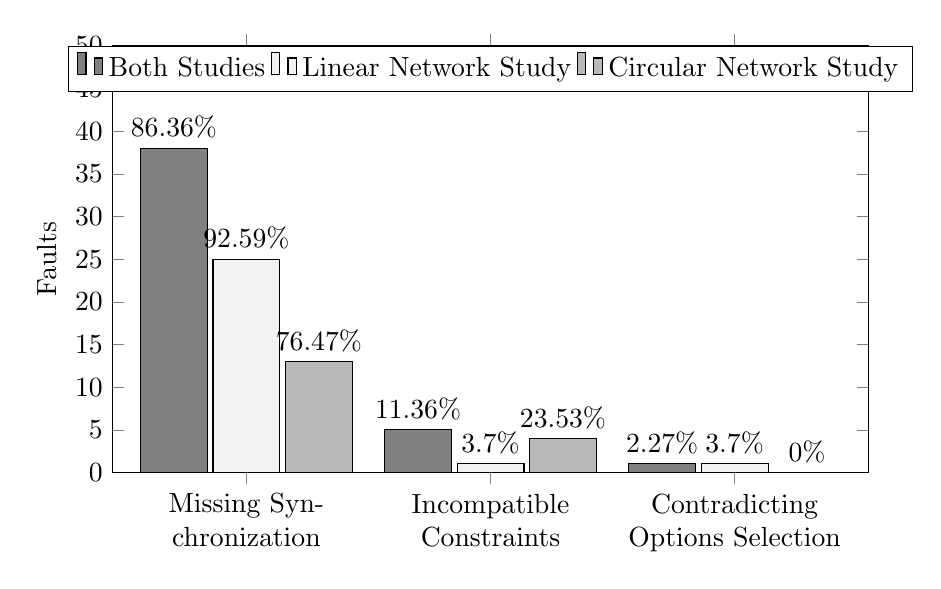
\begin{tikzpicture}
    \begin{axis}[
        ybar,
        bar width=0.85cm,
        x=3.1cm,
        height=7cm,
        legend style={at={(0.5,1)},anchor=north,legend columns=-1},
        ylabel={Faults},
        symbolic x coords={Missing Synchronization, Incompatible Constraints, Contradicting Options Selection},
        xticklabel style={text width=2.8cm, align=center},
        xtick=data,
        ytick distance=5,
        ymin=0,
        ymax=50,
        enlarge x limits={abs=1.7cm},
        nodes near coords align={vertical},
    ]
    \addplot[fill=gray,
        point meta={y*100/44}, % 44 Mistakes in total, calculate percentage
        nodes near coords={\pgfmathprintnumber\pgfplotspointmeta\%},
        ] table[x=Mistake Type, y=occurrences, col sep=comma] {
            Mistake Type,                       occurrences
            Missing Synchronization,            38
            Incompatible Constraints,           5
            Contradicting Options Selection,    1
        };
    \addplot[fill=gray!10,
        point meta={y*100/27}, % 27 Mistakes in total, calculate percentage
        nodes near coords={\pgfmathprintnumber\pgfplotspointmeta\%},
        ] table[x=Mistake Type, y=occurrences, col sep=comma] {
            Mistake Type,                       occurrences
            Missing Synchronization,            25
            Incompatible Constraints,           1
            Contradicting Options Selection,    1
        };
    \addplot[fill=gray!55,
        point meta={y*100/17}, % 17 Mistakes in total, calculate percentage
        nodes near coords={\pgfmathprintnumber\pgfplotspointmeta\%},
        ] table[x=Mistake Type, y=occurrences, col sep=comma] {
            Mistake Type,                       occurrences
            Missing Synchronization,            13
            Incompatible Constraints,           4
            Contradicting Options Selection,    0
        };
        \legend{Both Studies, Linear Network Study, Circular Network Study}
    \end{axis}
\end{tikzpicture}
    \caption[Number of occurrences of mistake types]{Absolute numbers of faults due to different mistake types in both case studies. Percentages are relative to total number of faults in the particular case study.}
    \label{fig:correctness_evaluation:errors:mistake_type_numbers}
\end{figure}

\mnote{Relevance of mistake types}
Most importantly, we aimed to identify the relevance of the different types of mistakes according to \autoref{eq:categorization:relevance} by counting the numbers of faults they caused in our case studies.
We summarize the results of this analysis, depicting the evaluation of the according metrics, in \autoref{fig:correctness_evaluation:errors:mistake_type_numbers}.
We found that most faults were caused by missing synchronization.
Across both studies, more than \SI{85}{\percent} of the faults were caused by missing synchronization and even if only considering the circular network study they still made up more than \SI{75}{\percent} of all faults.
Incompatible constraints led to the second highest numbers of faults, namely about \SI{10}{\percent} when considering both case studies and about \SI{25}{\percent} when only considering the circular network study.
Finally, the contradicting selection of options only led to a single fault in the linear network study.

\mnote{Avoidance by construction}
The actual numbers must be assumed to be rather imprecise due to the low numbers of faults.
For example, only five faults due to incompatible constraints were detected in total.
Nevertheless, the relations between the numbers of fault occurrences show that missing synchronization was by far the most important reason for faults in transformations.
Since synchronization can be achieved by construction without knowing about the other transformations in a transformation network, this indicates that most errors in transformation networks can already be avoided by construction of the individual transformations.
Incompatibilities, as the reason for the second highest number of faults, can at least be analyzed when developing the transformation network, which means that it can at least be detected at design time without and before productively executing the transformations.

% Relevance: Most relevant is synchronization, then compatibility, option selection occurred seldom and not other problems in case study
% Although no option selection mistake in different, larger study, there was one in the first, only considering bidirectional transformations. Thus, we can expect this to be relevant for networks as well, even if it did not occur in the case study.
% In answer to \autoref{eq:categorization:relevance}, we can see that missing synchronization is the most relevant mistake type, followed by incompatibilities.
% Most importantly, mistakes that we can avoid by construction without knowing about the concrete network a transformation is used in are most important to avoid because they occur most frequently.

%\subsubsection{Orchestration}

\mnote{Relevance of orchestration problem}
Finally, we also aimed to evaluate the relevance of the orchestration problem in practice.
We have discussed that its evaluation is directly related to completeness of our categorization, because if we are able to classify each failure and trace it back to a fault covered by our categorization, there are no failures actually caused by the orchestration problem.
Since we were able to resolve all failures by fixing mistakes covered by our categorization, undecidability of the orchestration problem did not lead to the situation that the \vitruv framework was no able to find a consistent orchestration in any scenario.
Consequently, the according metric measuring the fail ratio evaluates to $0$:
\begin{align*}
    \mathvariable{fail\ ratio} = 0
\end{align*}

\mnote{Simple orchestration strategy sufficiency}
In particular, we selected a simple recursive strategy for the orchestration, which was still able to always find a consistent orchestration.
In answer to \autoref{eq:orchestration:relevance}, this indicates that the order in which transformations are executed may not be that relevant in practice, thus leading to the orchestration problem not being particularly relevant in practice.
We must, however, consider that the orchestration problem is especially relevant if multiple options for preserving consistency exists, like we have discussed as a possible restriction in \autoref{chap:orchestration:decidability:restriction}.
We have, however, seen that contradicting selection of options to restore consistency was not even a relevant fault in the case study, which may indicate that it is either not that problematic in practice or that the case study does not contain many cases in which multiple options for restoring consistency exist.

% Since we were able to categorize all occurring mistakes as consequences of actual mistakes that could have been avoided by proper construction or by analysis of the transformation, according to the identified mistakes types, and since all failures could be avoided when fixing the implementation faults as consequence of the mistakes, the transformation network was able to process all tested changed.
% In consequence, the simple orchestration strategy was able to find consistent orchestrations in all cases.

% In particular, if we consider that the strategy was very simple and was still able to find consistent orchestrations, at least in this case study the orchestration problem is not problematic.
% In fact, the fail ratio we wanted to consider to evaluate how often the algorithm fails because of the orchestration problem in \autoref{eq:orchestration:relevance} is zero.


\subsubsection{Synchronization}

\mnote{Synchronization approach correctness}
Most faults in both case studies were caused by missing synchronization.
In total, $38$ faults led to $214$ failures, and even if only considering the circular network study, still $13$ faults could be identified.
We were able to fix all these faults by adding matchings for existing elements by both explicit and implicit unique information, i.e., using correspondences as well as key information, as proposed in \autoref{chap:synchronization:achieving:identification}.
Thus, all $214$ scenarios which failed due to missing synchronization, i.e., mistakes at the \leveltransformation level, and in which we were able to apply our approach, succeeded after applying the proposed approach for constructing a synchronizing transformation by matching elements.
Thus, our approach operates correctly according to \autoref{eq:synchronization:correctness}, as its application always leads to correct synchronizing transformations in the case study, as reflected by the success ratio metric:
\begin{align*}
    \mathvariable{success\ ratio} = 1
\end{align*}

\mnote{Synchronization approach completeness}
In addition, we were able to apply our approach in all cases in which faults at the \leveltransformation level led to failures during execution.
More precisely, there we no cases in which we were not able to perform matching of elements due to unique information, thus requiring us to use heuristics and having the possibility to fail.
Additionally, there we no failures due to missing synchronization that occurred for other reasons than missing element matchings.
This indicates completeness of our proposed approach according to \autoref{eq:synchronization:completeness}, as there are no cases in which the approach could not be applied and resolve failures due to faults at the \leveltransformation level, which is also reflected by the according metric:
\begin{align*}
    \mathvariable{application\ ratio} = 1
\end{align*}

\mnote{Synchronizing transformation by construction}
%In addition to the metrics applied to the fixes during the case study, 
We have used the transformation between \gls{PCM} and \gls{UML}, which already applied our approach for matching existing elements to achieve a synchronizing transformation by construction.
Since we detected no failures due to missing synchronization of that transformation in either of the case studies, it serves as an additional indicator for the correctness and completeness of the approach, in addition to the measured metrics.

\mnote{Avoidance by construction}
In conclusion, we found the proposed approach for constructing synchronizing transformations to be correct and complete in the considered case studies.
This serves as an indicator for its general correctness and completeness, and thus the possibility to use it as a constructive approach for achieving synchronizing transformations.
Since we found missing synchronization to be the most important reason for failures in transformation networks, concluding that we can achieve synchronization by construction means that we are able to avoid most of these failures by construction.

% As discussed before, at transformation level 13 mistakes were made of only considering the network study and in total 51 mistakes were made when considering both studies.
% They led to, in total, 211 failures.
% All of them were fixed by adding matching of existing elements by explicit or implicit unique information, as proposed in \autoref{chap:synchronization:achieving:identification}.
% This indicates that our approach is correct, as it fulfills the proposed property of resolving failures due to mistakes at the \leveltransformation level.
% In fact, the success ratio metrics used to measure the correctness of our synchronization approach according to \autoref{eq:synchronization:correctness} is $1$, because for all considered changes that led to failures because of \leveltransformation level mistakes, consistency could be preserved after applying the approach.

% Additionally, this shows that our approach could be applied in all cases in which failures occurred due to missing synchronization.
% Thus, there were no cases in which the approach could not be applied.
% This means that there were no cases in which no unique matching of elements could be performed.
% Additionally, there were no failures due to missing synchronization that occurred for other reasons than missing element matching.
% The application ratio to measure the applicability of our approach according to \autoref{eq:synchronization:applicability} is $1$.


\subsubsection{Topology Effects}

\begin{propertable}
    \rowcolors{1}{\firstlinecolor}{\secondlinecolor}
    \begin{tabular}{L{9.2em+0.6\difftoafiveimage}C{4.4em+0.1\difftoafiveimage}C{4.4em+0.1\difftoafiveimage}C{4.4em+0.1\difftoafiveimage}C{4.4em+0.1\difftoafiveimage}}
        \toprule
        \hspace{1em} \newline
            \hspace{4.5em+0.5\difftoafiveimage} \textbf{Phase $\rightarrow$} \newline 
            \hspace{5.5em} \newline
            \hspace{5.5em} \newline 
            \textbf{$\downarrow$ Mistake Type} & 
        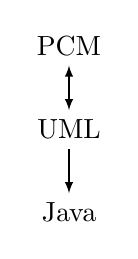
\begin{tikzpicture}
            \node[anchor=center] at (0,3em) (pcm) {\acrshort{PCM}};
            \node[anchor=center] at (0,0em) (uml) {\acrshort{UML}};
            \node[anchor=center] at (0,-3em) (java) {Java};
            \draw[latex-latex] (pcm) -- (uml);
            \draw[-latex] (uml) -- (java);
        \end{tikzpicture} & 
        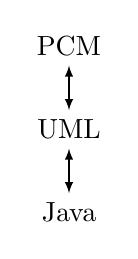
\begin{tikzpicture}
            \node[anchor=center] at (0,3em) (pcm) {\acrshort{PCM}};
            \node[anchor=center] at (0,0em) (uml) {\acrshort{UML}};
            \node[anchor=center] at (0,-3em) (java) {Java};
            \draw[latex-latex] (pcm) -- (uml);
            \draw[latex-latex] (uml) -- (java);
        \end{tikzpicture} & 
        \begin{tikzpicture}
            \node[anchor=center] at (0,3em) (pcm) {\acrshort{PCM}};
            \node[anchor=center] at (0,0em) (uml) {\acrshort{UML}};
            \node[anchor=center] at (0,-3em) (java) {Java};
            \draw[latex-latex] (pcm) -- (uml);
            \draw[latex-latex] (uml) -- (java);
            \draw[-latex] (pcm.west) -- ++(-0.7em-0.1*\difftoafiveimage,0) |- (java);
            %\draw[-latex] (pcm.north) |- ++(-2em,0.7em) |- ([yshift=-0.7em]java.south) -- (java);
        \end{tikzpicture} & 
        \begin{tikzpicture}
            \node[anchor=center] at (0,3em) (pcm) {\acrshort{PCM}};
            \node[anchor=center] at (0,0em) (uml) {\acrshort{UML}};
            \node[anchor=center] at (0,-3em) (java) {Java};
            \draw[latex-latex] (pcm) -- (uml);
            \draw[latex-latex] (uml) -- (java);
            \draw[latex-latex] (pcm.west) -- ++(-0.7em-0.1*\difftoafiveimage,0) |- (java);
        \end{tikzpicture} \\
        \midrule
        Incorrect transformation & 5 & 2 & 4 & 1 \\
        Missing synchronization  & 0 & 0 & 6 & 7 \\
        Incompatible constraints & 0 & 0 & 2 & 2 \\
        Incompatible options selection & 0 & 0 & 0 & 0 \\
        \bottomrule
    \end{tabular}
    \caption[Mistake types by case study phase]{Numbers of faults due to different mistake types by the phase of the circular network case study with the stepwise addition of unidirectional consistency preservation rules.}
    \label{tab:correctness_evaluation:errors:mistakes_by_phase}
\end{propertable}

\mnote{Mistake types per case study phase}
We have performed the circular network case study in a four-phase process, as explained at \autoref{fig:correctness_evaluation:errors:study_phases}, adding a unidirectional consistency preservation rule in each phase to analyze how the topology affects the types of faults that are revealed by failures when applying our test scenarios to the network of each phase.
We depict the numbers of faults as consequences of the different mistakes types in the different phases in \autoref{tab:correctness_evaluation:errors:mistakes_by_phase}.

\mnote{Incorrectness revealed by combination}
In the first two phases, the consistency preservation rules of the transformations between \gls{UML} and Java are added.
Since these two phases were already covered by the linear network study, it was likely that only few further faults are found by extending the test cases.
In this case study, we extended the test cases to also validate the generated Java model, whereas in the linear network case study the test cases validated only the \gls{PCM} and \gls{UML}, or the \gls{UML} and Java models, respectively, but not the third model.
Interestingly, in these phases only faults due to incorrect transformations were found as reasons for failing test scenario executions.
On the one hand, this shows that it seems to be difficult to construct correct transformations that consider all possible scenarios.
In this case, the combination of transformations to a network revealed incorrectness due to cases that were not considered for a transformation on its own before.
On the other hand, this indicates that it may already be sufficient to validate pairwise consistency of models in multiple scenarios when executing a transformation network, rather than validating consistency of all models, since no faults due to the combination of transformations to a network could be found in these phases.
As we have seen in the linear network study, such faults can actually occur already in a linear network.

\mnote{Cycles introducing synchronization errors}
As expected, in the last two phases especially faults due to missing synchronization are revealed by the occurring failures.
This is due to the reason that these phases introduce a cycle in the transformations, which leads to the situation that transformation need to synchronize changes, as both models may have been changed across two paths of transformation executions.
Even in these phases, failures occur due to incorrect transformations.

\mnote{Transformation correctness not assumable}
Thus, as the essential takeaway, it is important to not only consider mistakes specific to the combination of transformations to a network, but also to consider correctness of the individual transformations when constructing a transformation network.
The results of our case study indicate that assuming transformations to be correct may not be reasonable in practice, thus transformations may fail when combined to a network because of faults that they already contained before, but which never led to failures when executing them in an isolated way.


% The expected result is that synchronization mistakes first occurred when a cycle of the unidirectional transformations occurs which does not only consist of the cycle within one bidirectional transformations.
% Only in that setting a synchronization scenario occurs which requires transformations to consider that other transformations may have created elements in both models.
% Additionally, also errors at the network levels only occurred in those stages, although they could already occur in a linear network, like they also occurred in the single transformation case study, in which already the unidirectional consistency relations could be incompatible.

% We had to perform two iterations of the previously described process.
% In the first iteration, we faced failures due to mistakes at the operationalization level, whereas in the second iteration only failures due to remaining mistakes at the modularization level occurred.
% We have tagged the states before and after the evaluation process in the GitHub repository~\owncite{vitruvCBSEGithub}.

% \begin{copiedFrom}{ICMT}

%\compactsubsection{Classification}

% In the first iteration, all 187 tests failed.
% The reason was that all transformations assumed that new elements are only created by the user or the transformation itself.
% In consequence, we observed multiple instantiations and insertions in 187 cases, which we could trace back to 35 missing matchings of elements in the transformations.
% After adding appropriate matchings, all these failures disappeared in a second iteration, so for the first iteration $\mathit{identifiedFailureRatio = resolvedFailureRatio = 1}$, since all detected failures were identified and resolved.

% In the second iteration, 5 new failures occurred.
% Three of them were diverging loops, which were caused by a namespace repeatedly prefixed to the name of classes, interfaces and enumerations in Java.
% The causing mistakes were incompatible constraints: The Java model contains the fully qualified name of a class, whereas the UML model only contains the simple name, which was correctly propagated from UML to Java, but the namespace prefix was not removed in the opposite direction.
% The two other failures were alternating loops, which were caused by alternations of element visibilities.
% For methods and constructors, the visibilities were repeatedly changed due to an inconsistent mapping of visibilities from UML to Java and vice versa.
%After fixing the mistakes, two failures remained.
%Nevertheless, the reason for that were technical issues with the transformation engine due to its propagation of atomic changes.
%Since the original failures also disappeared in this case, we again have $identifiedFailureRatio = resolvedFailureRatio = 1$, since all detected failures were identified and resolved.
% After fixing those mistakes, no failures remained.
% So we again have $\mathit{identifiedFailureRatio = resolvedFailureRatio = 1}$, since all detected failures were identified and resolved. 

% Summarizing, we were able to classify and resolve all failures in the case study and trace them back to mistakes with our classification in \autoref{chap:errors}.
% This demonstrates the applicability of our categorization and is an indicator for the completeness and correctness of our catalog.
% Most important, we did not find any failures that were caused by mistakes at a different specification level than we expected.
% To further validate the catalog, we should apply it to further case studies.
% It is however hard to find existing, independently developed transformations between at least three metamodels.
% They would have to be developed in a schema similar to the one proposed by \textowncite{kramer2016c}.
%\todoHeiko{Irgendwie noch sagen, dass wegen das wegen dem hohen Aufwand kein Threat to Validity ist? Oder kommt das nicht gut an?}
%\todoHeiko{Generell mehr Threats to Validity diskutieren?}


% \todo{Erkennntis aus Iterationen: Solange wir nur einen Baum von Relationen haben, gibt es keine Fehler auf Modularisierungsebene (keine Inkompatibilitäten), diese kommen erst bei Zyklus hinzu (allerdings schon bei internem Zyklus durch Unidirektionalität?). D.h. wie schon voher angegeben sind Inkompatibilitäten per Konstruktion vermieden, wenn wir nur einen Baum von Relationen haben.
% Falls wir keinen Baum garantieren können: In this case, the consistency specifications must be revised whenever non-termination or non-deterministic termination of consistency preservation is observed (see \autoref{fig:correctness:categorization})}

%\compactsubsection{Element Matching}

%In \autoref{sec:avoiding:matching}, we presented three levels of matching equal elements across different transformation paths.
%We used our case study to investigate, which of those levels are necessary in a practical scenario.

% \end{copiedFrom} % ICMT


\subsection{Discussion and Validity}

From the two discussed case studies, we can derive several important insights.
This covers correctness of our categorization and synchronization approach, as well as, and in particular, regarding the relevance of different mistake types and the relevance of the orchestration problem.

\subsubsection{Insights}

\mnote{Most faults avoidable by construction}
We found that most faults in the case study were due to missing synchronization.
Synchronization is, however, achievable by construction, as we have also validated in the case study.
The proposed approach for synchronizing transformations can be applied to a single transformation without knowing about the other transformations to combine it with.
In consequence, a high number of faults in transformation networks can already be avoided by construction of the single transformations.

\mnote{Synchronization faults hide others}
In the iterative process of the case studies, we found that the first occurring failures were multiple instantiations because of missing synchronization.
Adding the element matchings for synchronization then revealed further faults, for example, because of incompatible relation.
First, this is not surprising, because multiple instantiation occurs upon creation of elements, which is the first step in consistency preservation.
Thus, faults due to missing synchronization lead to early failures.
Second, this shows that faults due to missing synchronization can hide further faults.
Thus, it is important to resolve errors at the \leveltransformation level first, or, in the best case, avoid them by construction.

\mnote{Multiple instantiation by incompatible relations}
In the circular network study, we detected multiple instantiations due to incompatible consistency relations rather than missing synchronization.
We have discussed in \autoref{chap:errors} that this can, theoretically, be the case, but still multiple instantiations are expected to be the consequence of missing synchronization in most cases.
While this is still given in the case studies, we also found that two kinds of multiple instantiation can be distinguished to identify their cause.
In case of missing synchronization, an element with the same key information, such as the name or other information, is created.
For matching existing elements, we proposed to use unique key information, such as names, to identify the existence of an element.
On the contrary, if the elements differ in their key information but still should be the same, there is a fault in the transformations in terms of incompatible consistency relations, as they use different ways of relating the key information, although it should actually be the same.

\mnote{Relevance of orchestration problem}
Finally, we found undecidability of the orchestration problem not to be relevant in our case studies.
This does not validate that it is not relevant in practice at all, but at least serves as an indicator that it is not such a central problem that transformation networks are unlikely to ever work properly.
Still, external validity of that statements has to be improved by further studies.

%Central: Most mistakes can be avoided by construction!

%Erkenntnis: Multiple Instantiation kann auch durch andere Fehler auftreten, dann sind die Elemente aber unterscheidbar, da die Key-Information, die zur Synchronisierung genutzt wird, verschieden ist -> super für die Praxis.

%Erkenntnis: Immer erst Fehler auf Transformationsebene fixen, da diese Fehler auf den anderen Ebenen verdecken.

%In Timurs MA außerdem betrachtet wie sich eine Kategorisierung in too many, incorrect and too few elements auf failures auswirkt. Hieraus konnten jedoch keine relevanten Erkenntnisse gezogen werden, weshalb wir es hier nicht diskutieren und auf die MA verweisen (Table 5.2)


\subsubsection{Threats to Validity}

\mnote{Results indicate statement}
In the following, we discuss different possible threats to the validity of the discussed results.
%Due to the limited set of case studies, which especially limits external validity, all results can only be seen as indicators for the statements that we make.
The limited set of case studies especially limits external validity. %, all results can only be seen as indicators for the statements that we make.
We discuss how we have mitigated validity threats and for which reasons validity of the statements may be actually restricted, distinguished by construct, internal, conclusion and external validity~\cite{wohlin2012validity-Book}. %, i.e., how the case study setup may conflict with the proposed cause-effect relationships, and how the results generalize.

\paragraph{Construct Validity}
%The case study setup may not be representative to actually draw the given conclusions for different reasons.
\mnote{Pre-alignment of transformations}
If transformations are in some way aligned with each other a priori, certain errors would not occur at all, thus reducing the number of faults and influencing their distribution.
%We assumed the transformations not to be aligned with each other a priori, because otherwise certain errors would not occur at all, thus reducing the number of faults and influencing their distribution.
We have %, however,
mitigated this threat by developing each transformation in an isolated project without knowing that it is supposed to be combined with other transformations, as well as by giving the development task to different, independent students.
The only bias may be that the author of this thesis supervised the students that developed the different transformations.
Still, this is a situation comparable to practice, because the developers may also exchange information, but at least not have an explicit representation of common knowledge.

\mnote{Language selection}
We employed the \reactionslanguage to implement the transformations.
The language may affect how likely specific faults are to be made.
For example, the language and the \vitruv framework it is embedded into use a delta-based approach to consistency preservation, which may already prevent problems that may occur with a state-based approach to consistency preservation.
We did, however, explicitly use a language that provides a rather low level of abstraction to reduce the chance that this influences how prone the implementations are to specific faults.
For example, using \gls{QVTR}, which already provides the ability to define keys for matching existing elements, would have prevented specific faults already by construction.

\paragraph{Internal Validity}

\mnote{Constructing vs. fixing synchronization}
Using transformations that were not initially synchronizing and fixing them during the case studies leads to two threats to validity. 
First, this process obviously leads to a high number of faults and failures due to missing synchronizing, which would not have been the case when using transformations that are synchronizing a priori.
Since we wanted to evaluate how important it is to have synchronizing transformations, this setup was reasonable.
Still and second, it would be valuable to conduct a case study in which transformations are already synchronizing.
This can give further and more precise insights regarding the relevance of the other types of faults and, more importantly, the process of fixing faults rather than avoiding them may introduce a bias.
When fixing the faults, additional fixes beyond the application of our synchronization approach may have been performed until the test scenarios succeeded, which cannot occur if transformations are already developed to be synchronizing.
We mitigated this threat by constructing at least one of the transformations to be synchronizing and found that it did actually not lead to any failures because of missing synchronization.
Still, we plan to perform an appropriate case study to further validate how well synchronization can be achieved by construction and how this influences the relevance of other mistakes, as we will discuss in \autoref{chap:correctness_evaluation:categorization:limitations}.

%Construct Validity % extent to which experiment setup reflects theory, influenced by participant treatment
%- Alignment der Transformationen: könnten vorher/ungewollt schon aneinander angepasst sein, daher wenig Fehler. kein Threat, wurde per Konstruktion ausgeschlossen. Allerdings Bias dadurch dass der Autor alle Implementierungen betreut hat. Allerdings wie in echt: Man tauscht sich aus, aber hat keine explizite Definition des gemeinsamen Verständnisses
% - Categorization/Orchestration: Hier wenig Optionsauswahl, d.h. in den meisten Fällen entscheiden sich die Transformationen für ein Element und hat keine Auswahl. Daher vielleicht wenige Fehler auf höheren Ebenen beobachtet und keine Probleme mit Orchestrierungsproblem und nicht dadurch, dass es generell kein Problem ist. Vielleicht ist das in anderer Studie viel schlimmer.
% Orchestration Problem: Vielleicht ist die Fallstudie zu sehr gestreamlined, insb. durch wenige Auswahlmöglichkeiten um Konsistenz herzustellen (siehe Option Selection Faults). Für externe Validität der Aussage müsste man sich weitere Studien anschauen, insb. solche wo es mehr Auswahlmöglichkeiten gibt. Wie schon vorher diskutiert ist aber insbesondere die Frage, ob es noch andere relevante Ursache dafür gibt, dass man keine konsistente Orchestrierung findet --> Future Work
% - Synchronization: The transformation were not constructed synchronizing, thus obviously many synchronization errors occur. If the scenario is foreseen, there may be much less errors at this level and more at the others -> need to perform further evaluation were developer know about necessity to use transformations in a network to properly construct them and then see how often that still fails. (future work, like before)

%Internal validity % result may indicate relationship, although there is none
% - Auswahl der Studis für Transformationserstellung
% - Synchronization: Fixing errors rather than avoiding them may be biased. Maybe without knowing we integrated further fixes that led to non-failing implementations. Thus need to perform evaluation where developers apply our approach (future work).
% - Synchronization: Bias Sprache. Vielleicht sind die Reactions so, dass bis auf Element Matching alles richtig funktioniert, was in anderen Sprachen nicht so ist. Insb. wenn nicht delta-based gearbeitet wird. Daher waren durch Sprachauswahl gewisse Probleme nicht da, die bei anderen Sprachen vorkämen, und nicht weil sie gar nicht existieren.
% - Synchronization: Studie hatte immer eindeutige Key-Informationen. Daher möglicherweise deswegen anwendbar und nicht weil der Ansatz vollständig ist. Andere Studien ohne Key Informationen, falls es das gibt. Allerdings ist das essentielle Komplexität, die durch keinen Ansatz umgangen werden kann. Wenn es keine Informationen gibt um Elemente zu identifizieren ist es egal, ob man die anderen Transformationen kennt oder nicht. Man hätte dann lediglich die Möglichkeit Transformations-übergreifende Trace-Links zu verwenden, um das Problem zu umgehen, da diese dann die nötigen Key-Informationen an die Trace Links statt die Elemente heften.

\paragraph{Conclusion Validity}
\mnote{Amount of data}
The central threat to conclusion validity is the low amount of data.
Some fault types occurred only once in the case studies, thus potentially reducing the significance of the results.
This especially means that the actual values, especially for the relevance of the mistake types, cannot be considered representative.
Still, we expect the general conclusions regarding relevance to be correct, because the number of test scenarios was high enough and led to a significant number of failures.

%Conclusion Validity % draw conclusion about relationships, e.g., not enough data
% Threat due to few data. Only few faults in the studies. Thus the precise values are not reliable.
% Still, we expect the conclusion regarding the relevance of the mistake types to be correct.
% Same regarding other ratios, but only the fault values are low. We have a high number of test cases and of occurring failures, so no threat.

%External Validity % generalizability, improved by making environment more realistic%

\paragraph{External Validity}
\label{chap:correctness_evaluation:categorization:discussion:limitations}

\mnote{Number of case studies}
External validity in terms of generalizability of the results is especially affected by the representativeness of the case studies.
To this end, a threat may be the low number of performed case studies.
%Only two studies with the same sets of transformations may reduce generalizability.
%While in general other studies may be semantically different, they still only consist of models and transformations.
Our results are, however, not highly dependent on the actual contents of a case study, i.e., the contents of the models and the transformations, but rather dependent on the existence of specific patterns, such as the possibility for transformations to select from multiple options to restore consistency, and potentially from the size of a transformation network.
Especially the evidence of our results regarding relevance of faults at the \levelnetworkrule level needs to be further validated in additional case studies.
This is, however, difficult due to the limited availability of evaluation scenarios.
Regarding the size of transformation networks, we do not expect larger networks to reveal further problems, because the problematic situations are those in which changes to the same models are performed across two paths of transformation executions, which already exist with a cycle of three transformations.
In addition, only the number of case studies is rather low, but the number of considered scenarios within the case studies represents a comprehensive set of scenarios.

% Even having more than three transformations, we would assume the case of three transformation to generalize to an arbitrary number, because problematic are the situations in which information comes from two paths, which is already given with one cycle, thus inductively applied with more transformations and cycles.
% Real limitation is the low number of options in the consistency relations, which may be different in other scenarios, thus leading to other relevance of mistake type or even to mistakes and faults that we have not yet foreseen.
% To this end, we can only improve evidence in the generalizability of our results by performing further case studies with different transformation networks.
% This is, however, difficult due to limited ability. Still, this is a topic for future work.

\mnote{Scenario selection}
The selection of scenarios for the case studies may have influenced whether specific kinds of mistakes can occur at all.
In particular, the used transformations can all rely on unique key information for identifying matching elements.
Thus, we may have identified the synchronization approach to be correct and complete because the case study scenarios do not reflect problematic cases.
This is, however, essential complexity that cannot be solved with any comparable approach, because if no unique key information exists, only heuristics to identify elements can be applied.
To circumvent that problem, it would only be possible that transformations know each other and use trace links generated by the other transformations, such that they can rely on meta data attached to these links to uniquely identify elements.
This does, however, break the assumption of independent development and thus cannot be achieved by construction of a single transformation, but essentially requires transformations to be aligned with each other or to be defined as multidirectional transformations.

\mnote{Limited options in consistency relations}
Finally, the consistency relations in the case studies do not provide many different options for models to be consistent.
Thus, the chance that transformations decide to use different, contradictory options to restore consistency may be unlikely.
This may have led to only few faults, especially at the \levelnetworkrule level, and thus biased the results.
It does especially also influence the ability that undecidability of the orchestration problem leads to a failure.
It is, however, also a consequence of using a transformation language that does not explicitly define consistency relations that led to this result.
Since consistency relations are only implicitly defined by the consistency preservation rules, a contradictory selection of options manifests as an incompatibility of the implicit consistency relations, as the options to select from are not documented anyway.
Thus, to mitigate this issue, consistency relations would have to be defined explicitly.


\subsection{Limitations and Future Work}
\label{chap:correctness_evaluation:categorization:limitations}

In addition to the discussed results, the case studies also revealed some limitations of our approaches and insights, which represents our starting points for future work in terms of practical application improvements, conceptual progress and additional necessary evaluations.

% In \autoref{chap:correctness_evaluation:categorization:discussion:limitations}, we have discussed several limitations of our proposed approaches and current finding regarding synchronization of bidirectional transformations and the categorization of possible mistakes, faults and failures in transformations networks, which were especially revealed by the evaluation. 
% In the following, we discuss these opportunities for future work in terms of practical application improvements, conceptual progress and additional necessary evaluations.

\paragraph{Element Matching Implementation}
\mnote{Manual implementation}
Within the case studies, we have implemented the matching of existing elements manually, i.e., using the existing constructs provided by the transformation language.
This is a costly and cumbersome task, which is also prone to errors in the accidental complexity of the mechanism due to repetitions of the same logic.
Since the mechanism is always similar and only differentiates in the key information used to search for, it could be embedded into an \gls{API} or language construct to be reusable.

\mnote{Language-integrated synchronization}
In future work, we thus want to investigate how we can integrate the patterns for constructing synchronizing transformations into existing transformation languages, such as the \reactionslanguage used in the evaluation.
In particular, we want to investigate how well \gls{QVTR} fits for that purpose, as it already allows to define keys for matching existing elements~\cite[7.10.2.]{qvt}. % which represents the essential idea of the proposed approach.

\paragraph{Semantic Element Matching}
\mnote{Syntactic element matching}
In the evaluation, we have detected cases which may be expected to be consequences of incompatibilities, but are actually not.
For example, the transformation between \gls{UML} and \gls{PCM} creates a repository starting lowercase, whereas the transformation between Java and \gls{PCM} generates a repository starting uppercase.
Then the repository created by one transformation is not matched by the other, which is correct as the transformations define consistency relations with different capitalizations of the repository.
Thus, having two repositories is correct in this case, although it may not be expected, but intuitively would be assumed to be incompatible.
It is expected that both repositories are supposed to represent the same element (see~\owncite[Fig.~6.4]{saglam2020ma}), thus having the same semantics although their uniquely identifying information, the name, is not equal.
In this case, however, a different notion of correctness is violated that we explicitly excluded for this thesis in \autoref{chap:correctness:notions_correctness:dimensions}.
This notion assumes a common global knowledge to which the transformations must be correct, thus requiring knowledge about the semantics of the elements, for example, in terms of a global specification of consistency or a mapping to a common, verifiable formalism.

\mnote{Mapping to common formalism}
In future work, we want to consider how such a matching in terms of element semantics rather than plain syntactic matching can be performed. 
Although it requires the transformation developer to know about the semantics of the elements to define that they have to be syntactically matched, this process would be even more valuable if the matching was performed on more semantic information.
One such example that we have considered in \autoref{chap:compatibility} was the swap of first name and last name by one consistency relations, which does not represent an incompatibility according to our definition, but may intuitively be undesired.
Mapping all elements to a common semantic representation could improve such a matching process.
In \autoref{chap:improvement}, we will present an approach that proposes to describe transformations in terms of descriptions of the common elements of the metamodels, thus representing their common semantics.

% Erkenntnis: Was wir nicht ausschließen können sind Fehler in den Konsistenzrelationen, die auf der unterschiedlichen Interpretation von Konsistenz basieren. Wenn beispielsweise die Relation UML<>PCM das Repo klein schreibt, Java<>PCM aber das Repo groß schreibt, wird das (korrekterweise) nicht gematcht.
% Hier ist eine andere Auffassung von Korrektheit verletzt (Korrektheit der modularen bzgl. einer einheitlichen globalen Spezifikation), da implizit vorausgesetzt wird, dass in einem globale Verständnis in beiden Fällen auf das gleiche Repository abgebildet wird. (siehe Figure 6.4 in MA Timur).
% Dies war explizit nicht die Art von Korrektheit die wir betrachtet haben, da sie ein anderes Ziel verfolgt. Sie erfordert Kenntnis über die übergeordnete Semantik der Elemente, beispielsweise durch eine globale Konsistenzspezifikation, gegen die man das prüft (siehe entsprechendes Kapitel) oder durch die Abbildung auf einen gemeinsamen Formalismus, der verifizierbar ist.
% -> Semantisches Matching von Elemente (bzgl. zusätzlicher, darüberliegender Semantik) und nicht nur bzgl. irgendwelche Key-Werte. Das erfordert aber Abstimmung der Transformationen, Abbildung auf gemeinsamen Formalismus o.Ä. \autoref{chap:futurework:correctness:synchronization:semantic_matching}

\paragraph{Interaction with Users}
\mnote{Conflicts in consistency preservation rules}
In our assumptions in \autoref{chap:introduction:objective:assumptions}, we explicitly excluded semi-automatisms in consistency preservation from the considerations in this thesis.
Actual transformations can, however, be semi-automated by integrating decisions of users.
For example, a user may select whether an added class shall represent a component or not.
In terms of consistency relations, such decision options can be represented by multiple consistency relation pairs, representing all options to select from.
Within consistency preservation rules, such user decisions can, however, be problematic.
If both the transformation between \gls{UML} and \gls{PCM}, as well as between \gls{UML} and Java ask the user whether a class shall represent a component, this, on the one hand, is annoying if the user is asked twice and, on the other hand, can even lead to conflicting decisions by the user.
We have already discussed how the selection of different options by transformations can prevent the network from finding consistent models and in such a case, even worse, only one user decision can be correctly reflected in the result.
Thus, it is part of our future work to find out how to align user decisions across multiple transformations with each other.

% Erlaubt Java->PCM, dass man an beliebiger Stelle ein Interface anlegen kann. PCM-UML erlaubt das nur im contracts-Package. Erstellt man ein Interface in einem anderen Package, erstellt PCM-UML nochmal eines im contracts Package, dadurch auch UML-Java und dann matcht UML-PCM, wodurch es bei PCM-Java zwei Abbildungen des Interface gibt. Hier haben wir inkompatible Constraints, aber wenn die Nutzerabfrage für das Matching in beiden Transformationen PCM-Java und PCM-UML eingebaut wird, kann der Nutzer konfligierende Entscheidungen treffen. Um das zu verhindern, müssten die Transformationen aufeinander abgestimmt werden.
% Generell: Nutzerinteraktion lässt sich bei den Relationen dadurch ausdrücken, dass alle Auswahloptionen als valide consistency relation pairs betrachtet werden.
% Problematisch sind jedoch die consistency preservation rules, da sie es potentiell erlauben konfligierende der condition elements auszuwählen, genauso wie es bei den Transformationen selbst auch passieren kann.
% Wir haben diese selection of options im Orchestrierungs-Kapitel diskutiert.
% Hier ist definitiv noch Future Work notwendig um zu untersuchen, wie man Nutzerentscheidungen über mehrere Transformationen hinweg miteinander alignen kann \todo{Future Work}.
% Generell ist eine Untersuchung des Alignments von CPRs sinnvolles \todo{Future Work}.
% \autoref{chap:futurework:correctness:synchronization:user_interaction}

\paragraph{Alignment of Consistency Preservation Rules}
\mnote{Consistency preservation rule combination correctness notion}
We have made important insights regarding synchronization of transformations and compatibility, thus correctness at the \leveltransformation and \levelnetworkrelation levels.
At the \levelnetworkrule level, however, we only found the selection of contradicting options for consistency to be problematic, but we were neither able to restrict them without reducing expressiveness, nor to define any reasonable notion for correctness at all.
Thus, it remains an open question how consistency preservation rules need to be aligned with each other in a transformation network, such that a consistent orchestration of them always exists and, in the best case, that it can easily be found.
While finding a consistent orchestration is difficult due to undecidability of the orchestration problem anyway, in this thesis we focused on how to conservatively deal with this situation.
Although the evaluation indicated that the orchestration problem may not be highly relevant in practice, having a comprehensive, systematic theoretical understanding at that level, especially of how consistency preservation rules influence the ability to find consistent orchestrations and whether there are further issues except the selection of contradicting options would still be beneficial, which is why we consider it as important future work.

\paragraph{Synchronization Transformation Construction Case Study}
\mnote{Synchronization evaluation evidence}
Finally,  we have discussed two case studies to validate different properties of our proposed error categorization as well as the approach for constructing synchronizing transformations.
Although we were able to derive valuable conclusions, the case study was biased by the fact that two of three transformations were not designed to be synchronizing and, as part of the case study, fixed to be synchronizing during that study.
Still, it would be valuable to perform a case study with a focus on the construction of synchronizing transformations to improve evidence on the ability of correctly and completely achieving synchronizing transformations with our proposed approach.


%% COMBINED WITH FUTURE WORK
% \subsubsection{Limitations}

% In addition to the discussed results, the case studies also revealed some limitations of our approaches and insights, which represents our starting points for future work.

% \mnote{Implementation of element matching}
% Within the case studies, we implemented the matching of existing elements manually, i.e., using the existing constructs provided by the transformation language.
% This is cumbersome task, which is also prone to errors in the accidental complexity of the mechanism due to repetitions of the same logic.
% Since the mechanism is always similar and especially differentiates in the key information used to search for, it could be embedded in an API or language construct to be reusable.
% In future work we thus plan to integrate the approach to achieve synchronization of transformations into a language and validate its applicability, which we propose in \autoref{chap:futurework:correctness:synchronization:integration}.

% \mnote{Element matching by semantics}
% In the evaluation, we have detected cases which may be expected to be consequences of incompatibilities, but are actually not.
% For example, the transformation between \gls{UML} and \gls{PCM} creates a repository starting with lowercase, whereas the transformation between Java and \gls{PCM} generated a repository starting upper case.
% Then the repository created by one transformation is not matched by the other, which is correct as the transformations define consistency relations with different capitalizations of the repository.
% Thus, having two repositories is correct in this case, although it may not be expected, but intuitively would be assumed to be incompatible.
% Intuitively, it is expected that both repositories are supposed to represent them same element (see~\owncite[Fig.~6.4]{saglam2020ma}), thus having the same semantics although their uniquely identifying information, the name, is not equal.
% In this case, however, a different notion of correctness is violated that we explicitly excluded for this thesis in \autoref{chap:correctness:notions_correctness:dimensions}.
% This notion assumes a common global knowledge to which the transformations must be correct, thus requiring knowledge about the semantics of the elements, for example, in terms of global specification of consistency or a mapping to common, verifiable formalism.
% We aim to discuss such a correctness notion in future work (see \autoref{chap:futurework:correctness:synchronization:semantic_matching}).

% % Erkenntnis: Was wir nicht ausschließen können sind Fehler in den Konsistenzrelationen, die auf der unterschiedlichen Interpretation von Konsistenz basieren. Wenn beispielsweise die Relation UML<>PCM das Repo klein schreibt, Java<>PCM aber das Repo groß schreibt, wird das (korrekterweise) nicht gematcht.
% % Hier ist eine andere Auffassung von Korrektheit verletzt (Korrektheit der modularen bzgl. einer einheitlichen globalen Spezifikation), da implizit vorausgesetzt wird, dass in einem globale Verständnis in beiden Fällen auf das gleiche Repository abgebildet wird. (siehe Figure 6.4 in MA Timur).
% % Dies war explizit nicht die Art von Korrektheit die wir betrachtet haben, da sie ein anderes Ziel verfolgt. Sie erfordert Kenntnis über die übergeordnete Semantik der Elemente, beispielsweise durch eine globale Konsistenzspezifikation, gegen die man das prüft (siehe entsprechendes Kapitel) oder durch die Abbildung auf einen gemeinsamen Formalismus, der verifizierbar ist.
% % -> Semantisches Matching von Elemente (bzgl. zusätzlicher, darüberliegender Semantik) und nicht nur bzgl. irgendwelche Key-Werte. Das erfordert aber Abstimmung der Transformationen, Abbildung auf gemeinsamen Formalismus o.Ä. \autoref{chap:futurework:correctness:synchronization:semantic_matching}

% \mnote{Interaction with users}
% In our assumptions in \autoref{chap:introduction:objective:assumptions}, we explicitly excluded semi-automatisms in consistency preservation from the considerations in this thesis.
% Actual transformations can, however, be semi-automated by integrating decisions of users.
% For example, a user may select whether an added class shall represent a component or not.
% In terms of consistency relation, such decision options can be represented by multiple consistency relation pairs, representing all options.
% Within consistency preservation rules, such user decision can, however, be problematic.
% If both the transformation between \gls{UML} and \gls{PCM}, as well as between \gls{UML} and Java ask the user whether a class shall represent a component, this, on the one hand, is annoying if the user is asked twice and, on the other hand, can even lead to the user performing conflicting decisions.
% We have already discussed how the selection of different options by transformations can prevent the network from finding consistent models and in such a case, even worse, only one user decision can be correctly reflected in the result.
% Thus, it is part of our future work to find our how to align user decision across multiple transformations with each other (see \autoref{chap:futurework:correctness:synchronization:user_interaction}).

% % Erlaubt Java->PCM, dass man an beliebiger Stelle ein Interface anlegen kann. PCM-UML erlaubt das nur im contracts-Package. Erstellt man ein Interface in einem anderen Package, erstellt PCM-UML nochmal eines im contracts Package, dadurch auch UML-Java und dann matcht UML-PCM, wodurch es bei PCM-Java zwei Abbildungen des Interface gibt. Hier haben wir inkompatible Constraints, aber wenn die Nutzerabfrage für das Matching in beiden Transformationen PCM-Java und PCM-UML eingebaut wird, kann der Nutzer konfligierende Entscheidungen treffen. Um das zu verhindern, müssten die Transformationen aufeinander abgestimmt werden.
% % Generell: Nutzerinteraktion lässt sich bei den Relationen dadurch ausdrücken, dass alle Auswahloptionen als valide consistency relation pairs betrachtet werden.
% % Problematisch sind jedoch die consistency preservation rules, da sie es potentiell erlauben konfligierende der condition elements auszuwählen, genauso wie es bei den Transformationen selbst auch passieren kann.
% % Wir haben diese selection of options im Orchestrierungs-Kapitel diskutiert.
% % Hier ist definitiv noch Future Work notwendig um zu untersuchen, wie man Nutzerentscheidungen über mehrere Transformationen hinweg miteinander alignen kann \todo{Future Work}.
% % Generell ist eine Untersuchung des Alignments von CPRs sinnvolles \todo{Future Work}.
% % \autoref{chap:futurework:correctness:synchronization:user_interaction}

% \mnote{Alignment of Consistency preservation rules}
% Finally, we have made important insights regarding synchronization of transformations and compatibility, thus correctness at the \leveltransformation and \levelnetworkrelation levels.
% At the \levelnetworkrule level, however, we only found the selection of contradicting options for consistency to be problematic, but we were neither able to restrict them without reducing expressiveness, nor to define any reasonable notion for correctness at all.
% Thus, it remains an open question, how consistency preservation rules need to be aligned with each other in a transformation network, such that a consistent orchestration of them always exists and, in the best case, that it can easily be found.
% Although the evaluation indicated that this may not be a highly relevant practical problem, having a comprehensive theoretical understand at that level would also be beneficial, which is why we discuss it as future work in \autoref{chap:futurework:correctness:synchronization:cpr_alignment}.

% % Generell haben wir gute Erkenntnisse zu Synchronisation und Kompatibilität der Relationen, aber abgesehen von der Problematik der widersprüchlichen Optionsauswahl haben wir bzgl. der CPRs keine Erkenntnis gewonnen, wie diese inkompatibel sein können und daher verhindern, dass konsistente Modelle gefunden werden oder das Orchestrierungsproblem zuschlägt.
% % Das sollte in Future Work genauer geleuchtet werden. "Alignment of CPRs" \autoref{chap:futurework:correctness:synchronization:cpr_alignment}.